% Appendix A

\chapter{Appendix} % Main appendix title
\label{AppendixA} % For referencing this appendix elsewhere, use \ref{AppendixA}

\section{Choice of binning}
\label{sec:binning_optimization_study}

In this section, we show for few observables the unfolded results (considering only statistical uncertainty)
for a test setup and final setup for the \tty production and \tty prod+decay measurements. Additionally, we also show the migration matrix of events
from particle bin to reconstruction level in the signal region for the setups. In general no major differences are observed.

%%%% p_T(y)%%%
\begin{figure}[ht]
    \centering
    \subfloat[]{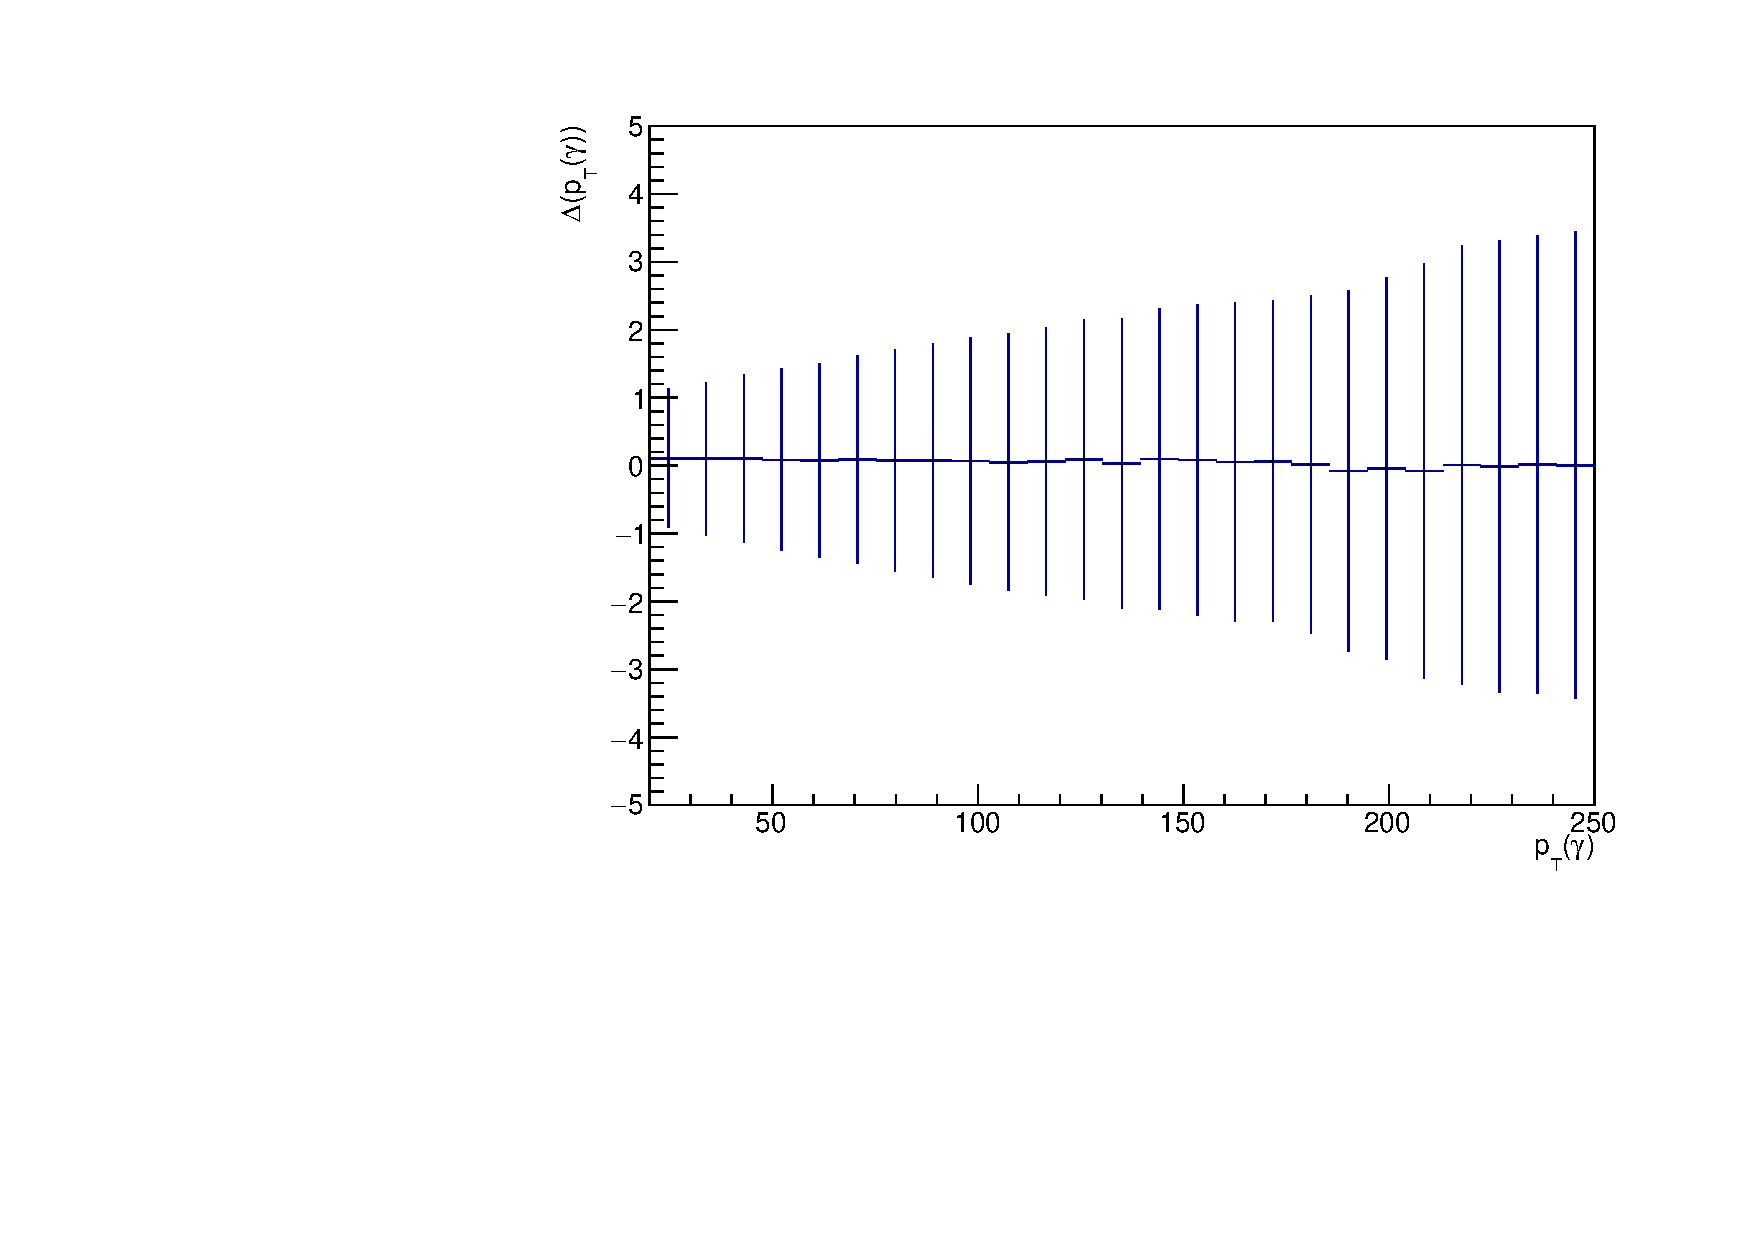
\includegraphics[width=0.4\textwidth]{figures/diff_xsec/binning_optimization/resolution/mean_stdDev_resolution_h2_ph_pt_reco_part_full_weighted.pdf}} \\
    \subfloat[]{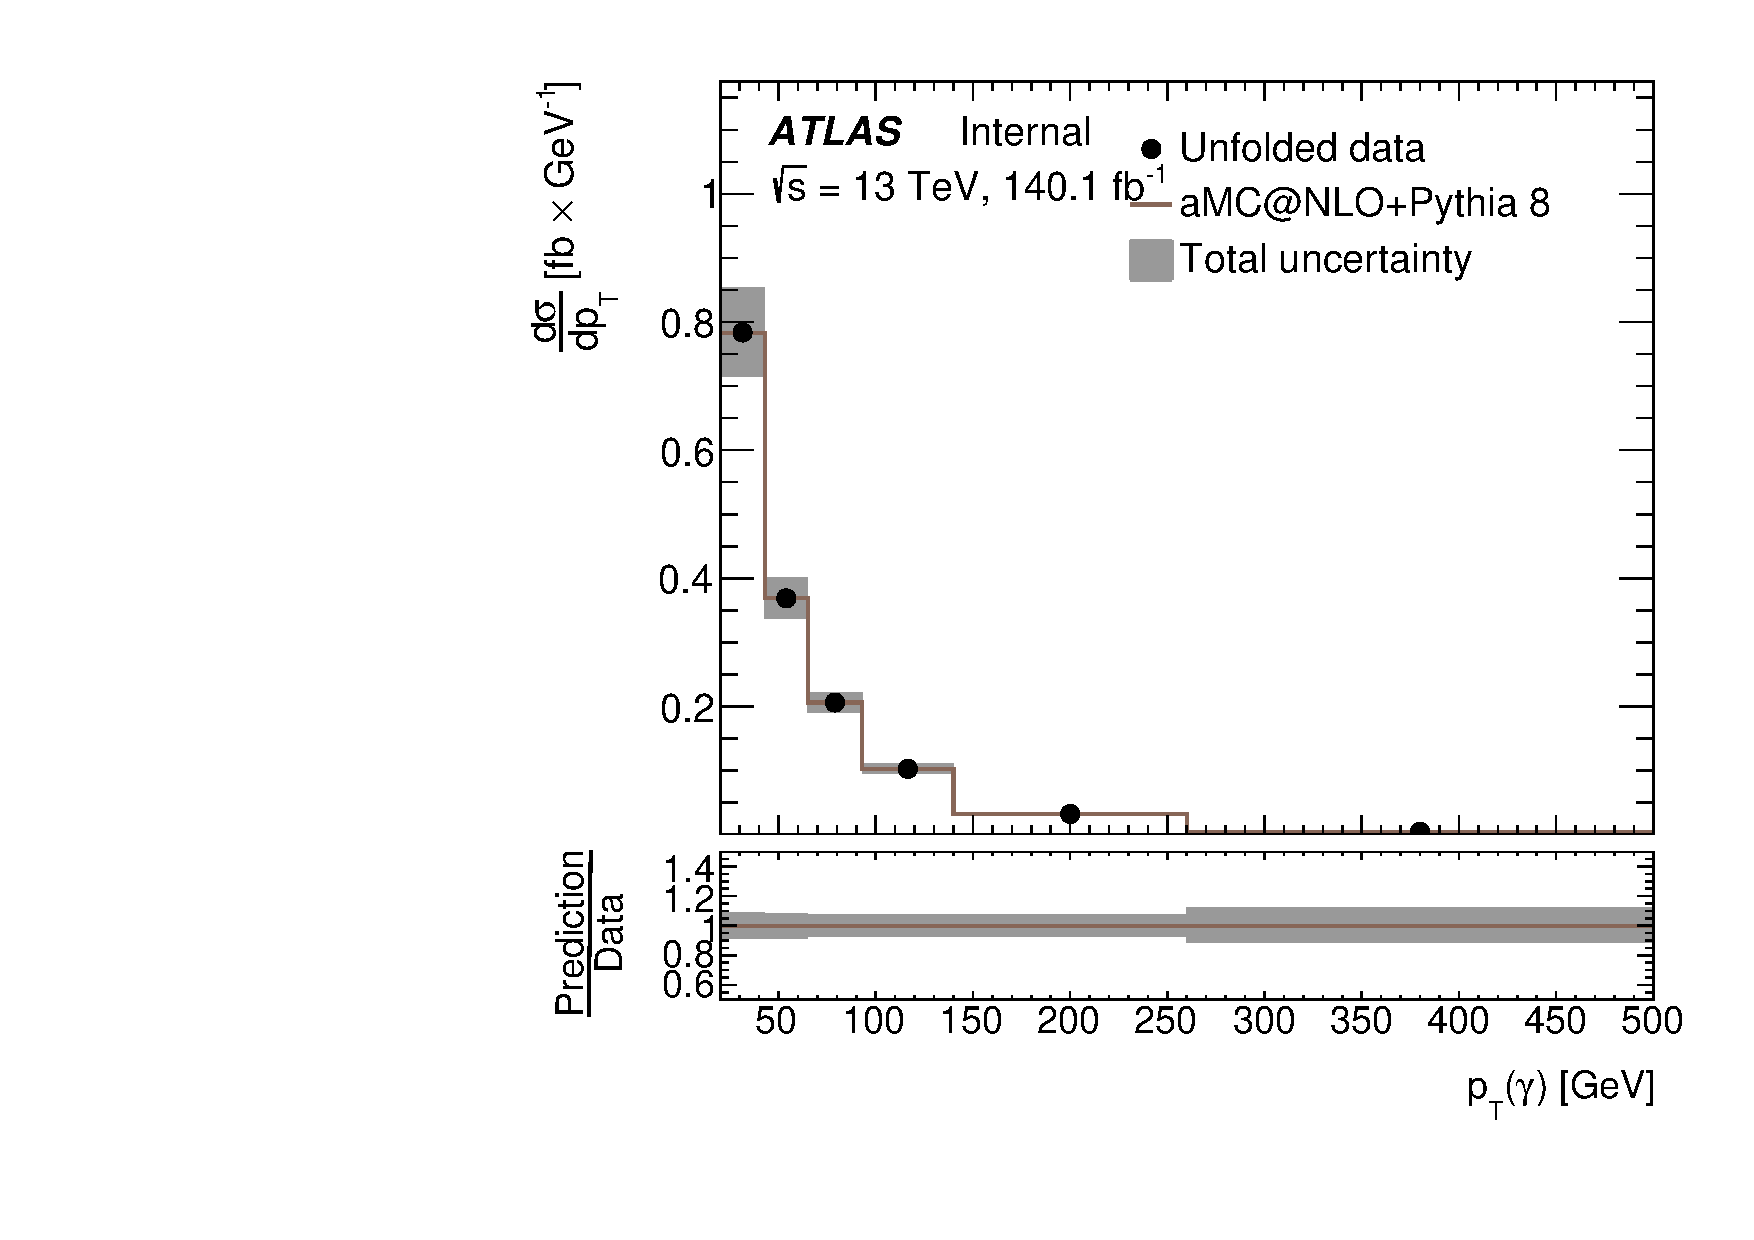
\includegraphics[width=0.23\textwidth]{figures/diff_xsec/binning_optimization/optimized_tty_prod/tty_pt_UnfoldedData.pdf}}
    \hfill
    \subfloat[]{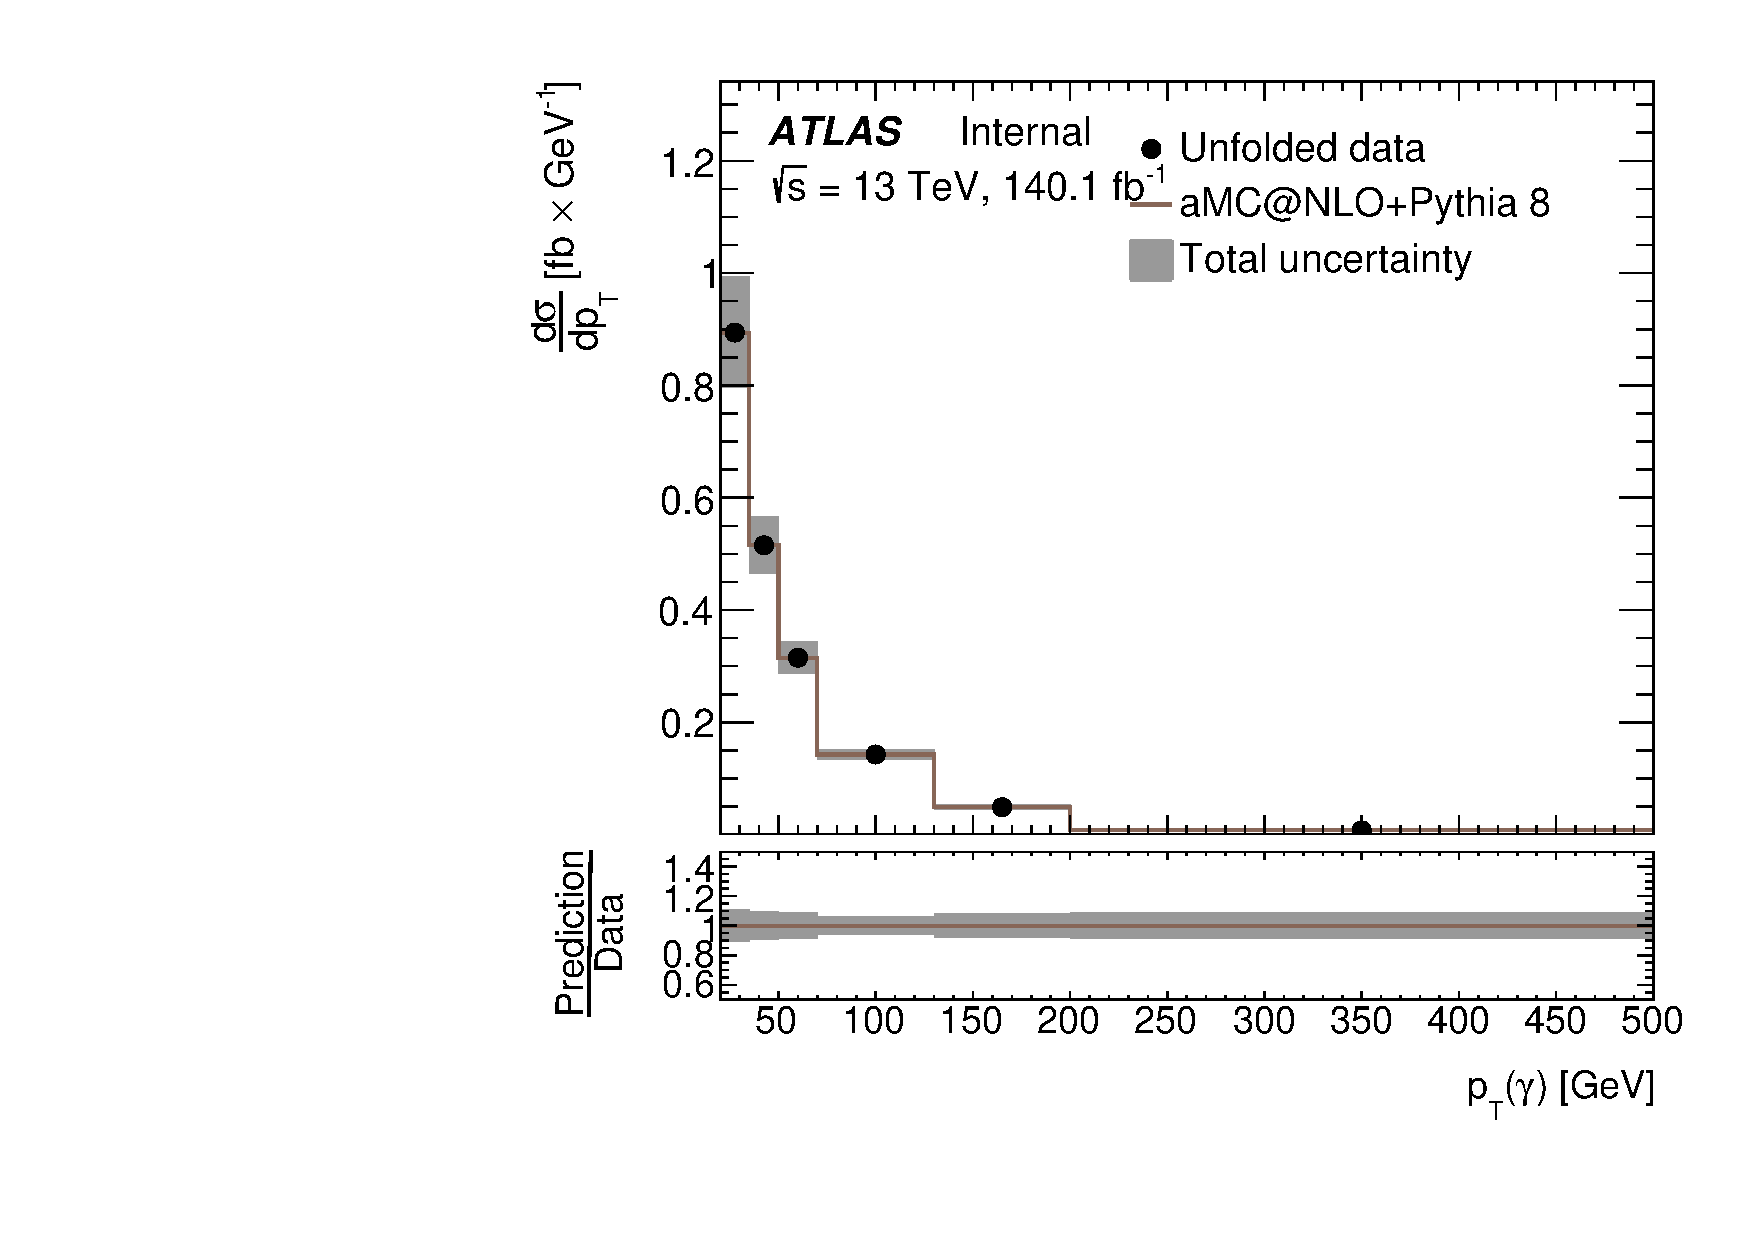
\includegraphics[width=0.23\textwidth]{figures/diff_xsec/binning_optimization/nominal_tty_prod/tty_pt_UnfoldedData.pdf}}
    \hfill
    \subfloat[]{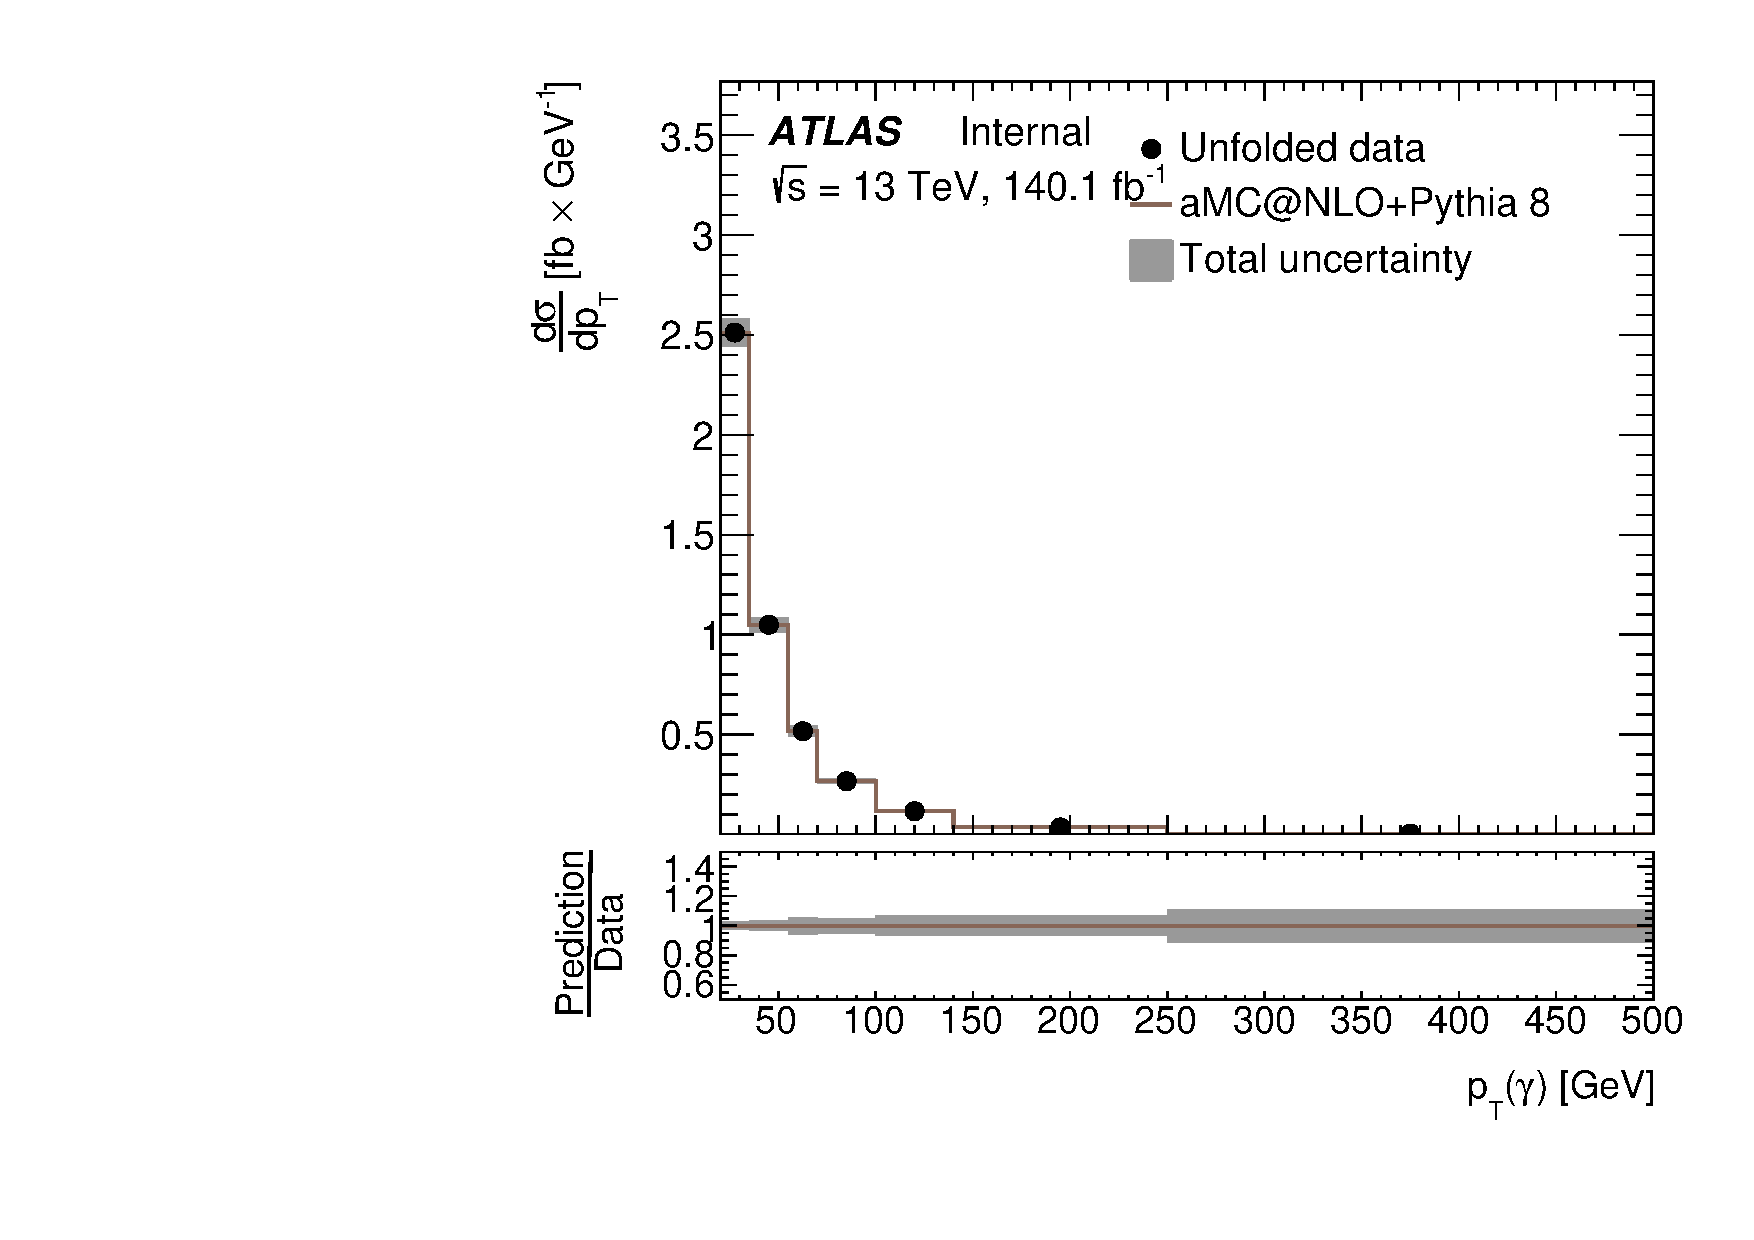
\includegraphics[width=0.23\textwidth]{figures/diff_xsec/binning_optimization/optimized_tty_incl/tty2l_pt_all_stat_UnfoldedData.pdf}}
    \hfill
    \subfloat[]{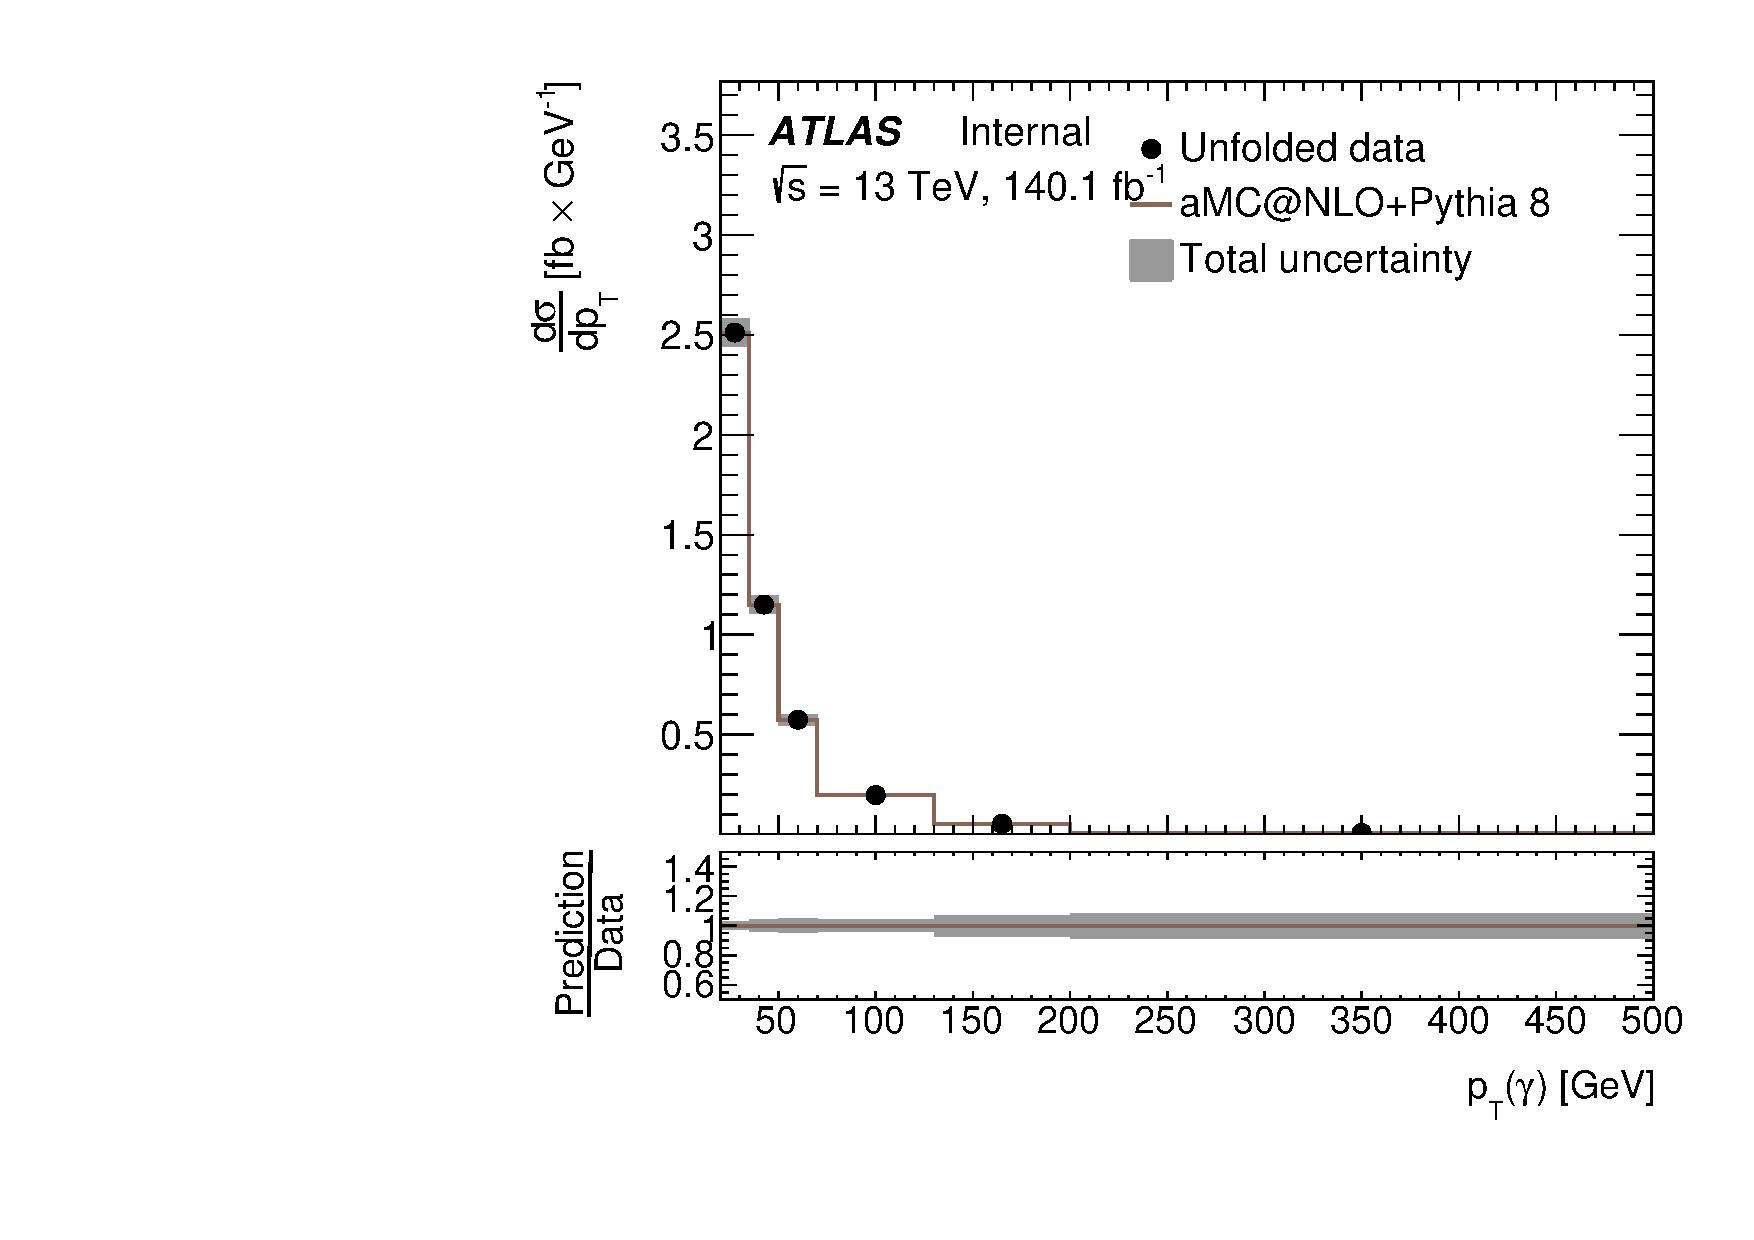
\includegraphics[width=0.23\textwidth]{figures/diff_xsec/binning_optimization/nominal_tty_incl/tty2l_pt_all_stat_UnfoldedData.pdf}}
    \hfill
    \subfloat[]{\includegraphics[width=0.23\textwidth]{figures/diff_xsec/binning_optimization/migrations/migration_tty_prod_06/migration_h2_ph_pt_reco_part_full_weighted_SR1.pdf}}
    \hfill
    \subfloat[]{\includegraphics[width=0.23\textwidth]{figures/diff_xsec/binning_optimization/migrations/migration_tty_prod_nominal/migration_h2_ph_pt_reco_part_full_weighted_SR1.pdf}}
    \hfill
    \subfloat[]{\includegraphics[width=0.23\textwidth]{figures/diff_xsec/binning_optimization/migrations/migration_tty_incl_06/migration_h2_ph_pt_reco_part_full_weighted_SR1.pdf}}
    \hfill
    \subfloat[]{\includegraphics[width=0.23\textwidth]{figures/diff_xsec/binning_optimization/migrations/migration_tty_incl_nominal/migration_h2_ph_pt_reco_part_full_weighted_SR1.pdf}}
    \hfill

    \caption{(a) Resolution of the photon $p_T$ observable is represented by the
    error bars. The y-axis is the mean of (reconstructed photon $p_T$ - truth
    photon $p_T)$ in GeV and the error bars represent one standard deviation
    around that mean. Unfolded results with the tested binning (b) and final
    binning (c) for \tty(prod) measurement and unfolded results with the tested
    (d) and final (e) binning for \tty(total) measurement, The error bar in (b),
    (c), (d), (e) represents statistical uncertainty only. Plots (f)- (i)
    represents the migration matrix in the SR for above cases.}
\end{figure}
\FloatBarrier

%%%% eta(y)%%%
\begin{figure}[ht]
    \centering
    \subfloat[]{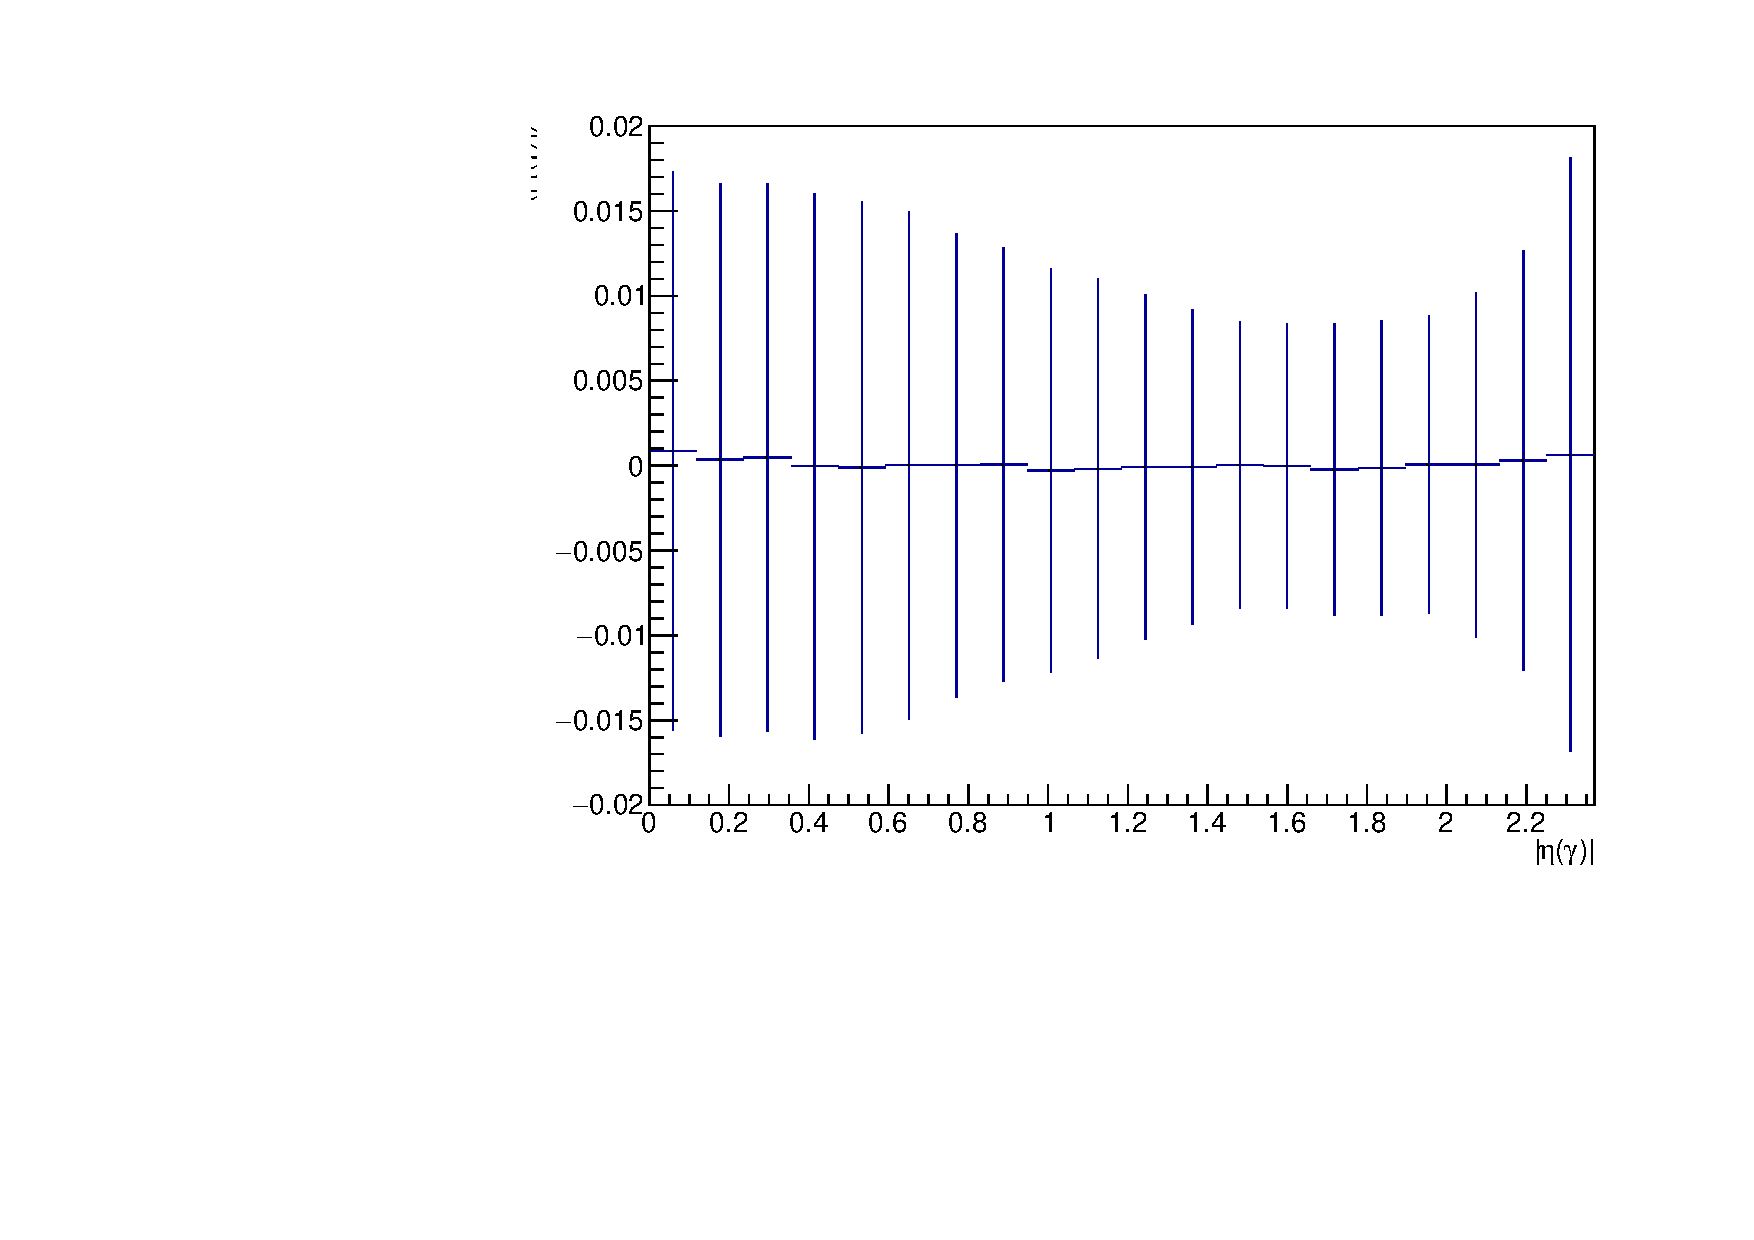
\includegraphics[width=0.4\textwidth]{figures/diff_xsec/binning_optimization/resolution/mean_stdDev_resolution_h2_ph_eta_reco_part_full_weighted.pdf}} \\
    \subfloat[]{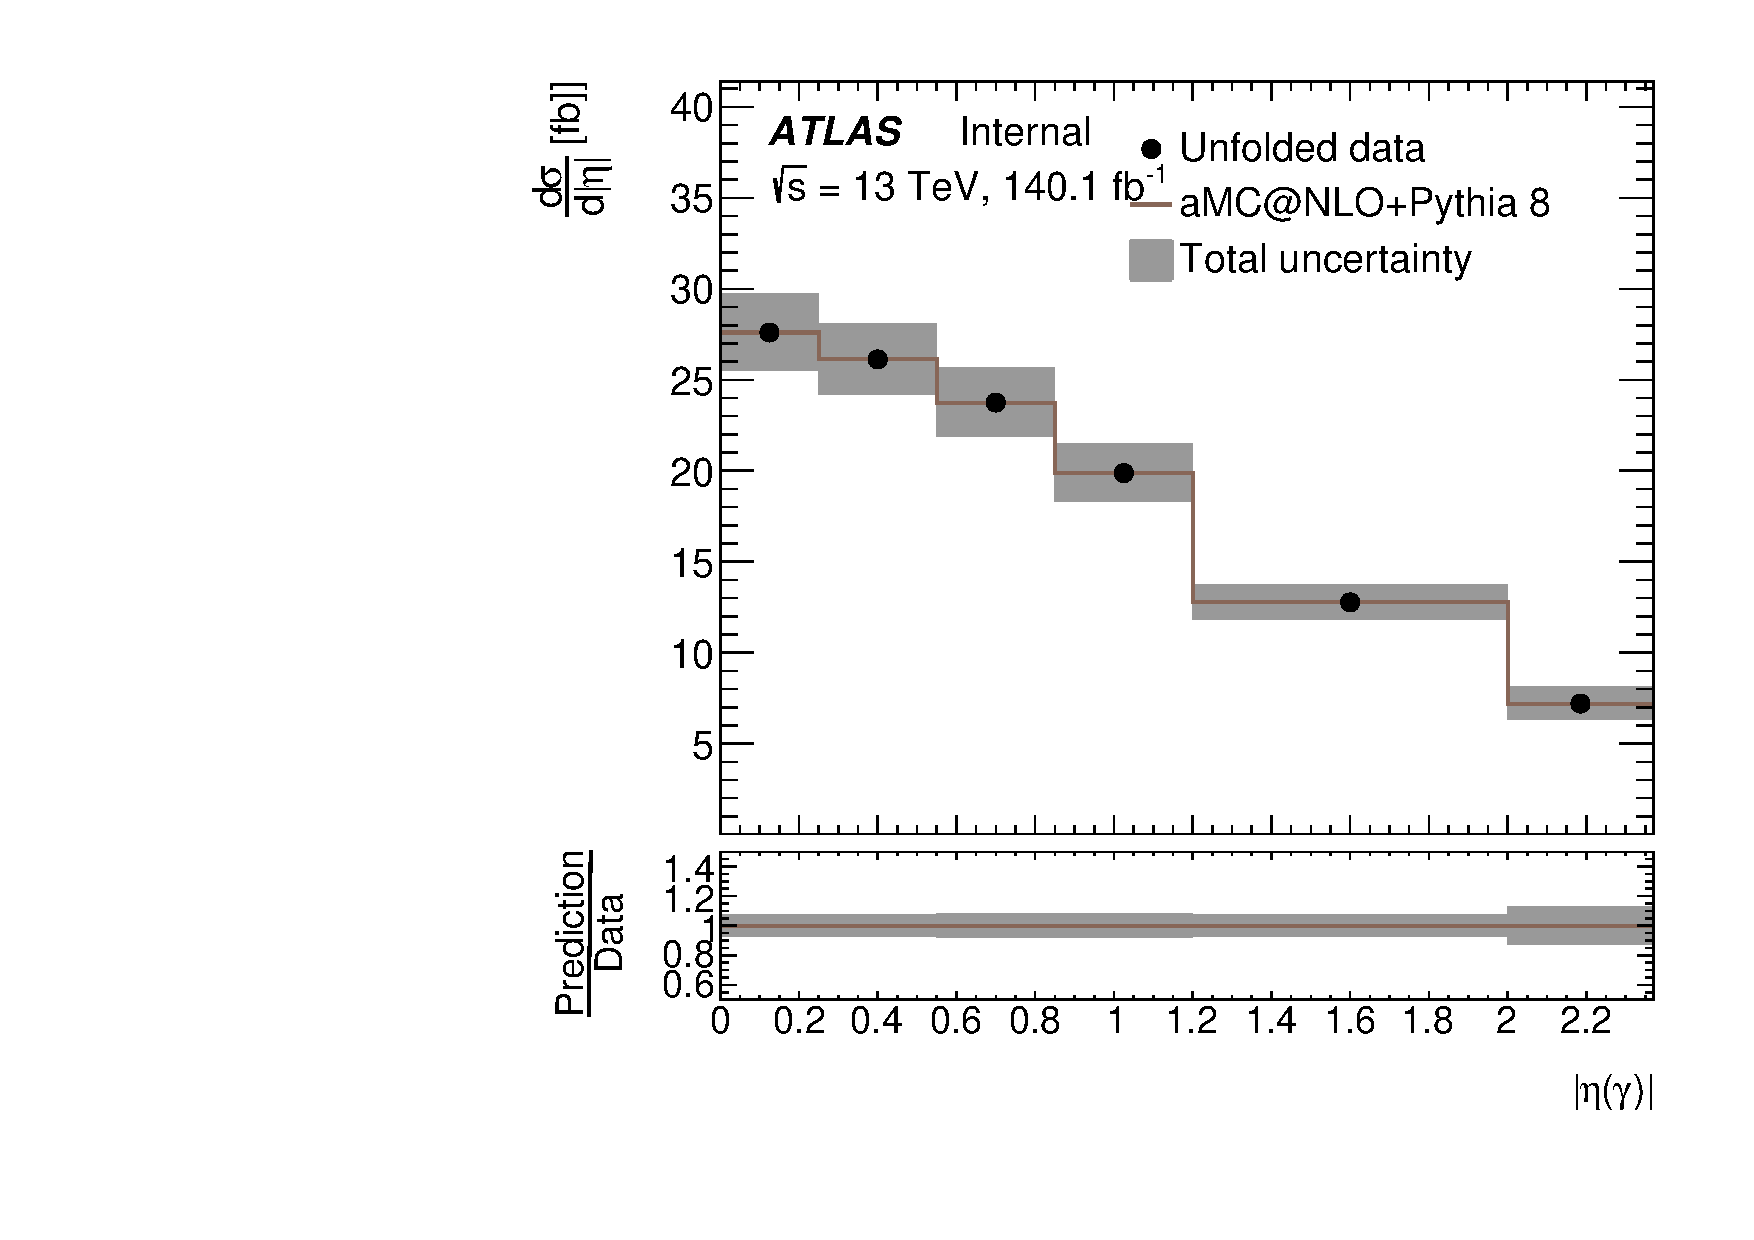
\includegraphics[width=0.23\textwidth]{figures/diff_xsec/binning_optimization/optimized_tty_prod/tty_eta_UnfoldedData.pdf}}
    \hfill
    \subfloat[]{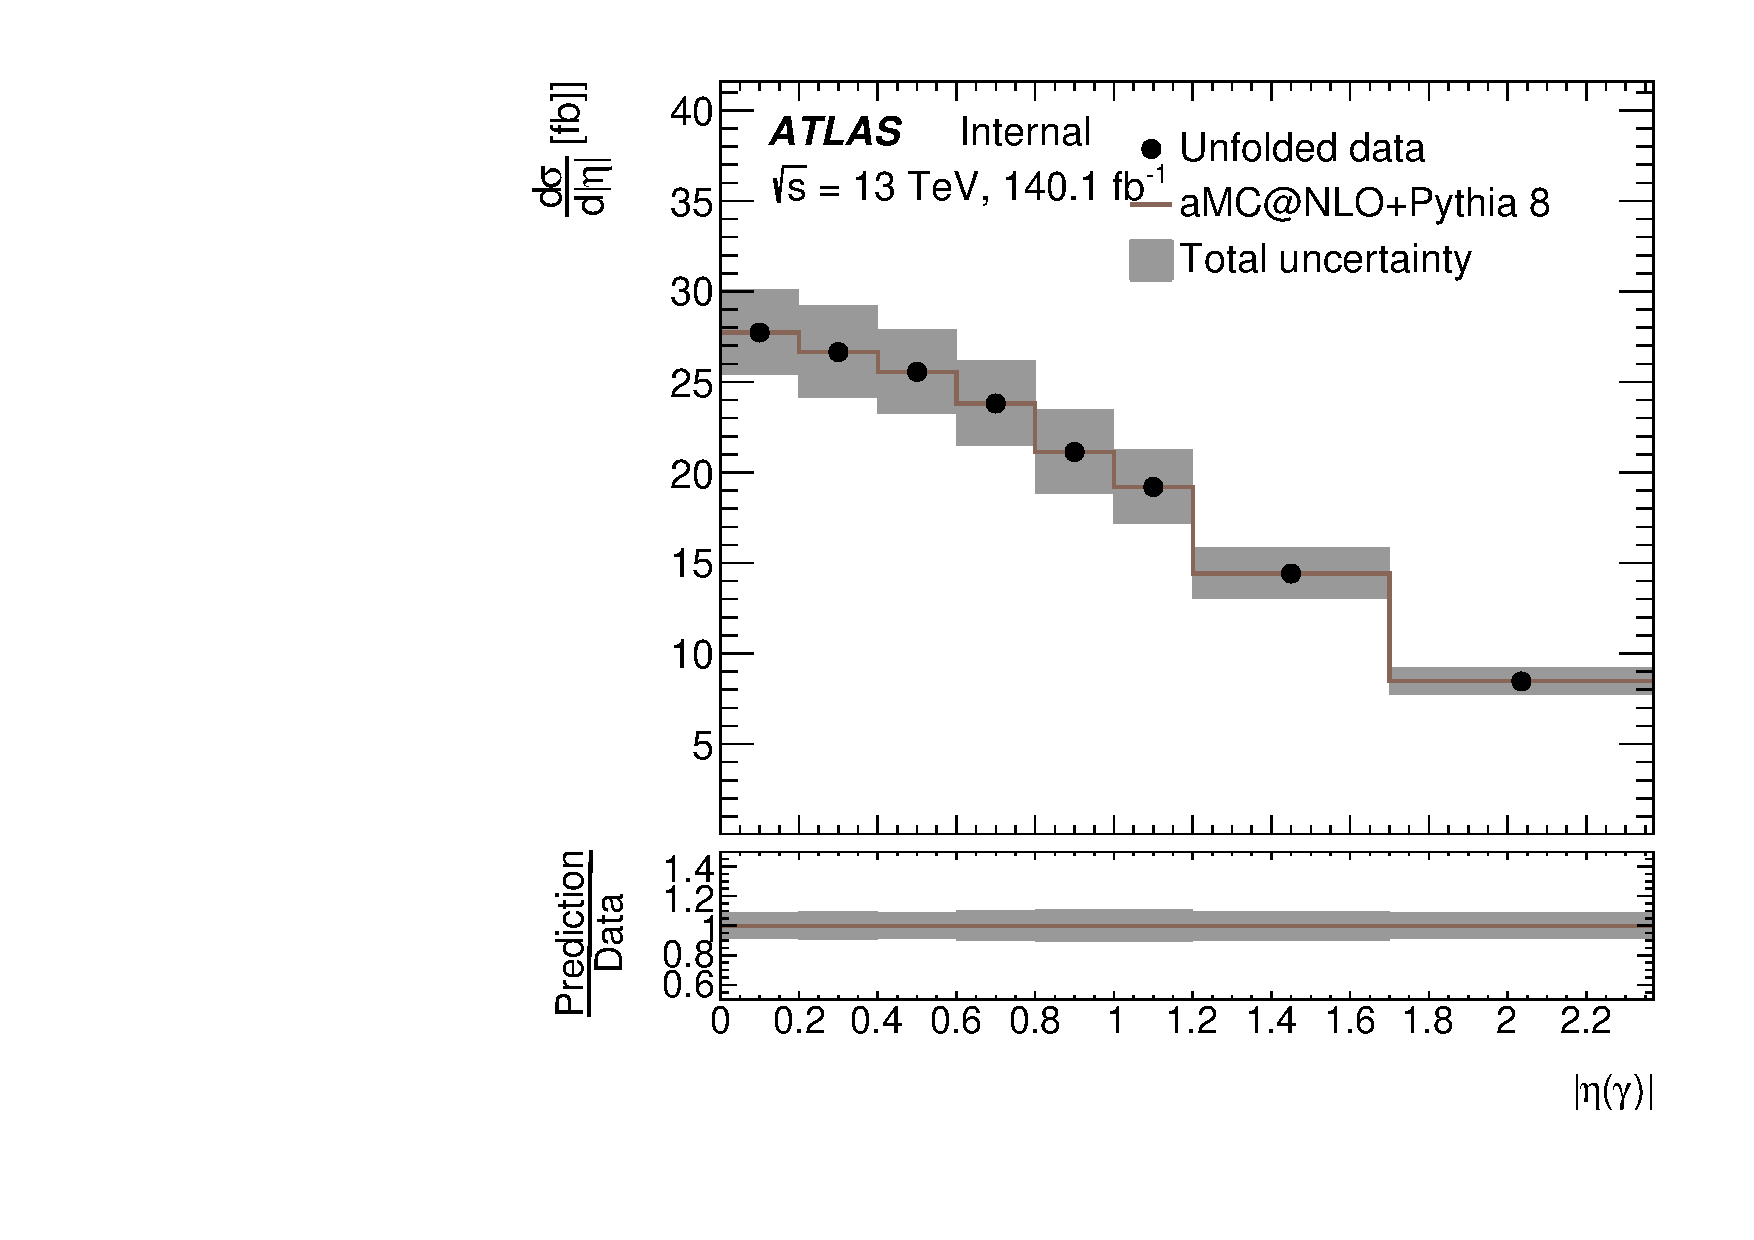
\includegraphics[width=0.23\textwidth]{figures/diff_xsec/binning_optimization/nominal_tty_prod/tty_eta_UnfoldedData.pdf}}
    \hfill
    \subfloat[]{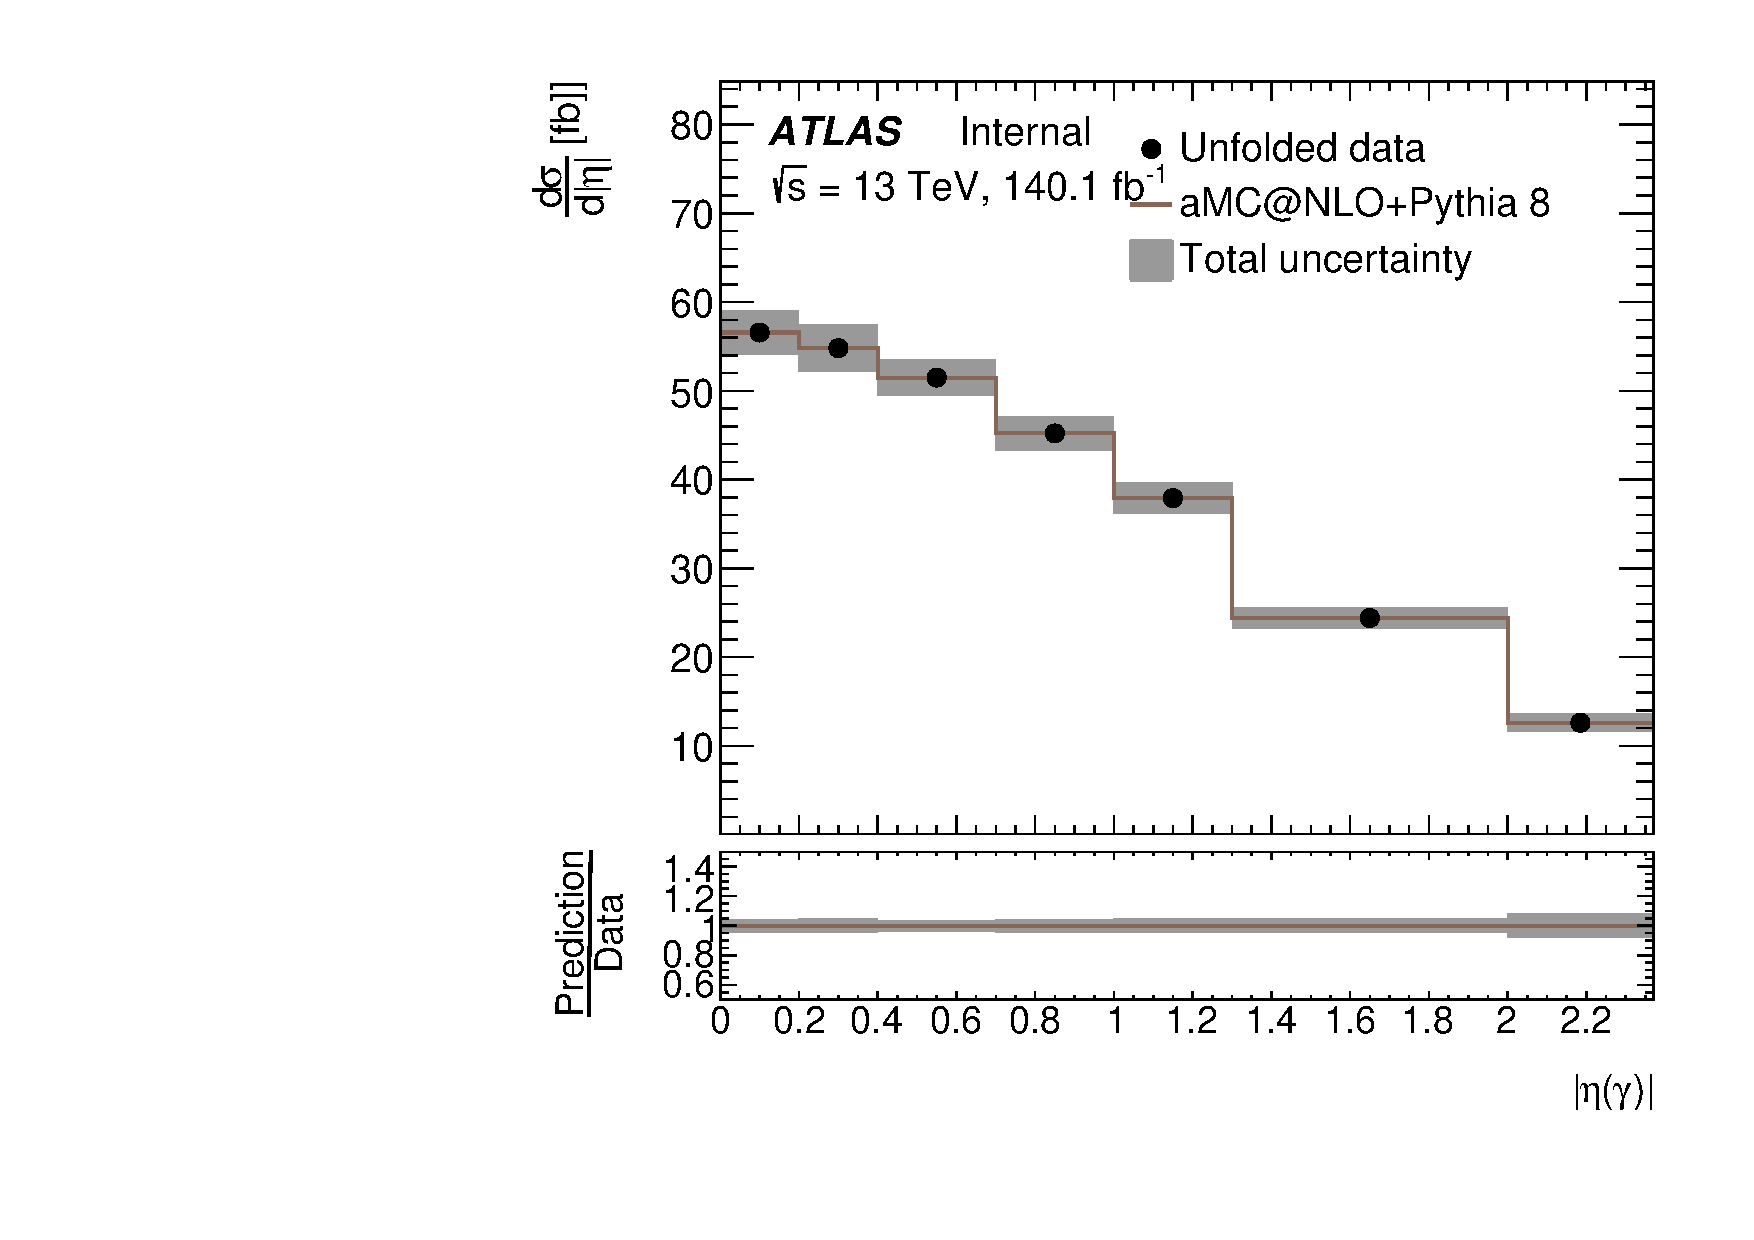
\includegraphics[width=0.23\textwidth]{figures/diff_xsec/binning_optimization/optimized_tty_incl/tty2l_eta_all_stat_UnfoldedData.pdf}}
    \hfill
    \subfloat[]{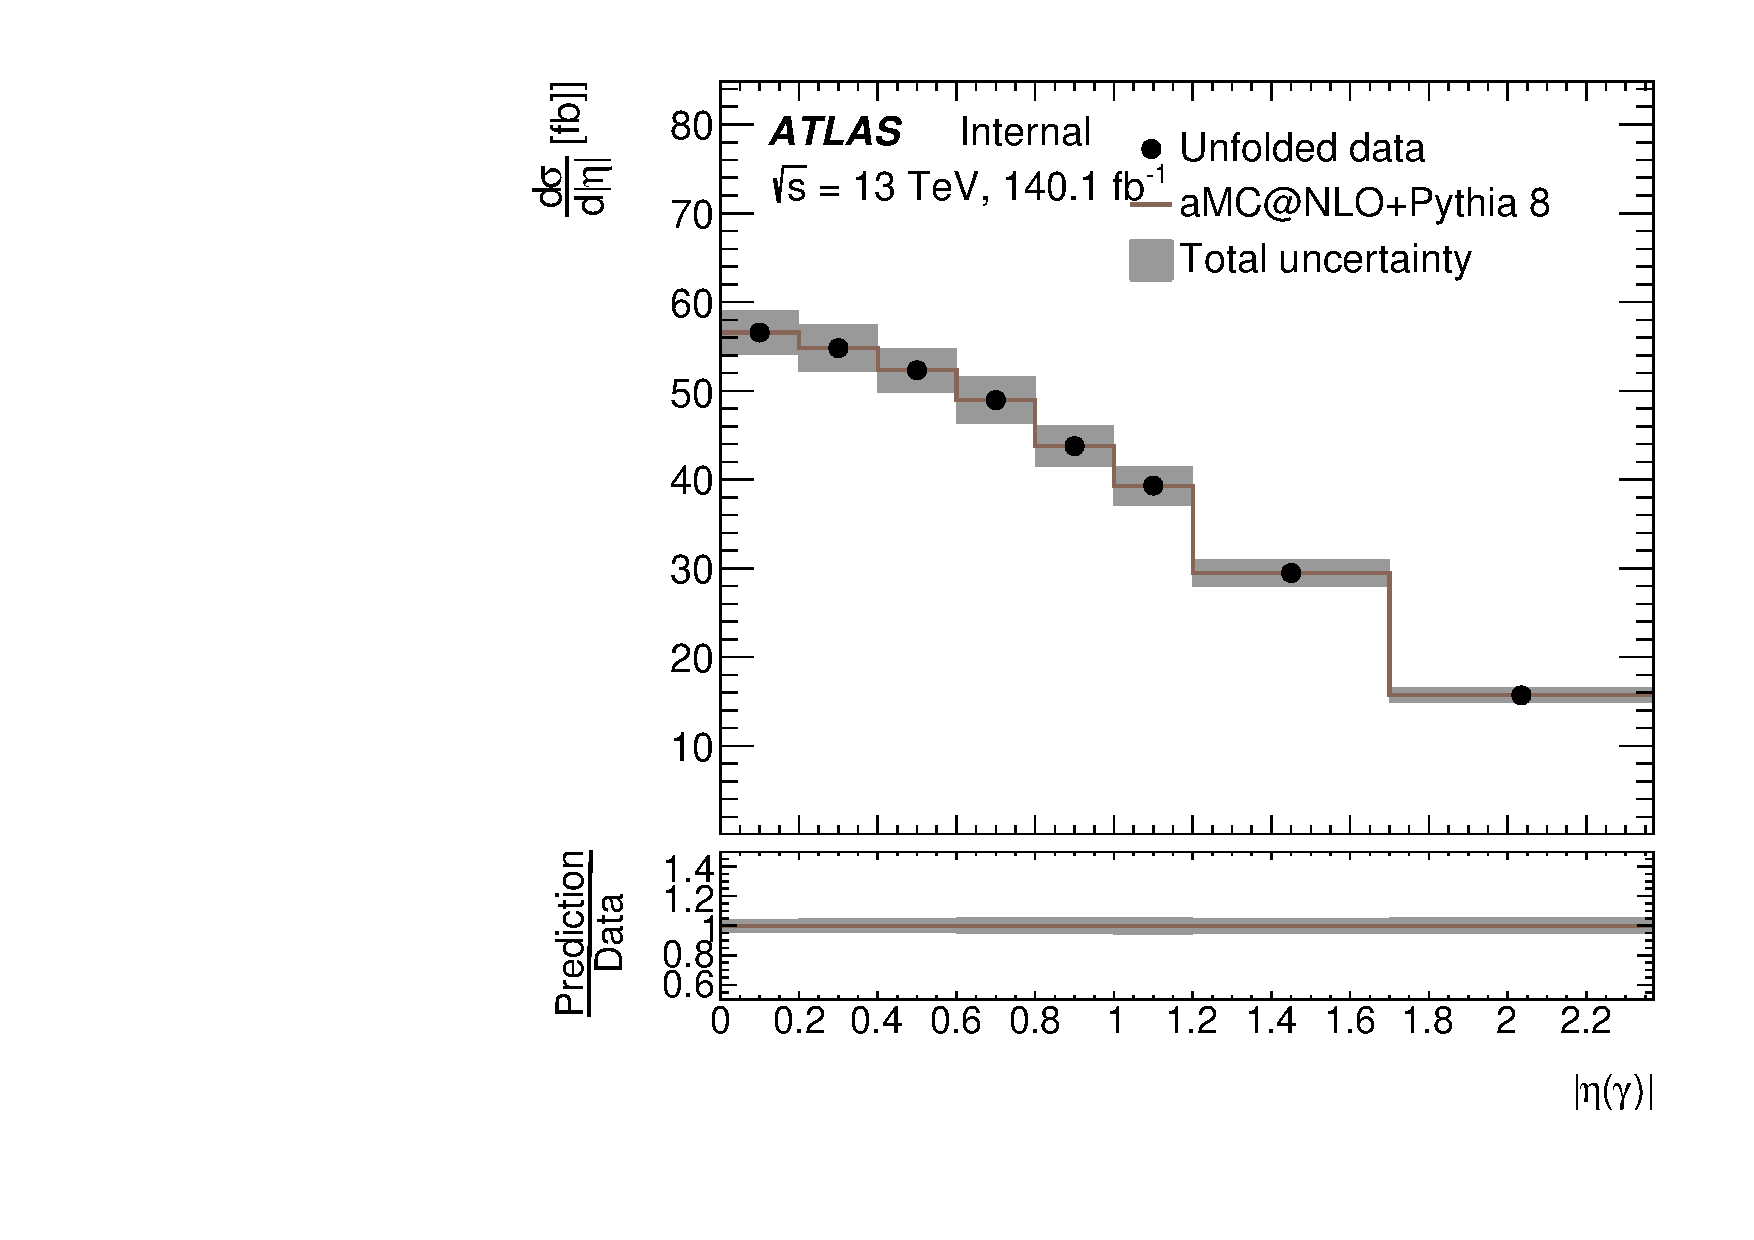
\includegraphics[width=0.23\textwidth]{figures/diff_xsec/binning_optimization/nominal_tty_incl/tty2l_eta_all_stat_UnfoldedData.pdf}}
    \hfill
    \subfloat[]{\includegraphics[width=0.23\textwidth]{figures/diff_xsec/binning_optimization/migrations/migration_tty_prod_06/migration_h2_ph_eta_reco_part_full_weighted_SR1.pdf}}
    \hfill
    \subfloat[]{\includegraphics[width=0.23\textwidth]{figures/diff_xsec/binning_optimization/migrations/migration_tty_prod_nominal/migration_h2_ph_eta_reco_part_full_weighted_SR1.pdf}}
    \hfill
    \subfloat[]{\includegraphics[width=0.23\textwidth]{figures/diff_xsec/binning_optimization/migrations/migration_tty_incl_06/migration_h2_ph_eta_reco_part_full_weighted_SR1.pdf}}
    \hfill
    \subfloat[]{\includegraphics[width=0.23\textwidth]{figures/diff_xsec/binning_optimization/migrations/migration_tty_incl_nominal/migration_h2_ph_eta_reco_part_full_weighted_SR1.pdf}}
    \hfill


    \caption{(a) Resolution of the photon $|\eta(\gamma)|$ observable is represented by the error bars. The y-axis
    is the mean of (reconstructed photon $|\eta(\gamma)|$ - truth photon $|\eta(\gamma)|$) in GeV and the error bars represent
    one standard deviation around that mean.
    Unfolded results with the tested binning (b) and final
    binning (c) for \tty(prod) measurement and unfolded results with the tested
    (d) and final (e) binning for \tty(total) measurement, The error bar in (b),
    (c), (d), (e) represents statistical uncertainty only.
    The error bar in (b), (c), (d), (e) represents statistical uncertainty only.
    Plots (f)- (i) represents the migration matrix in the SR for above cases.}
\end{figure}
\FloatBarrier

%%%% DR(y)%%%
\begin{figure}[ht]
    \centering
    \subfloat[]{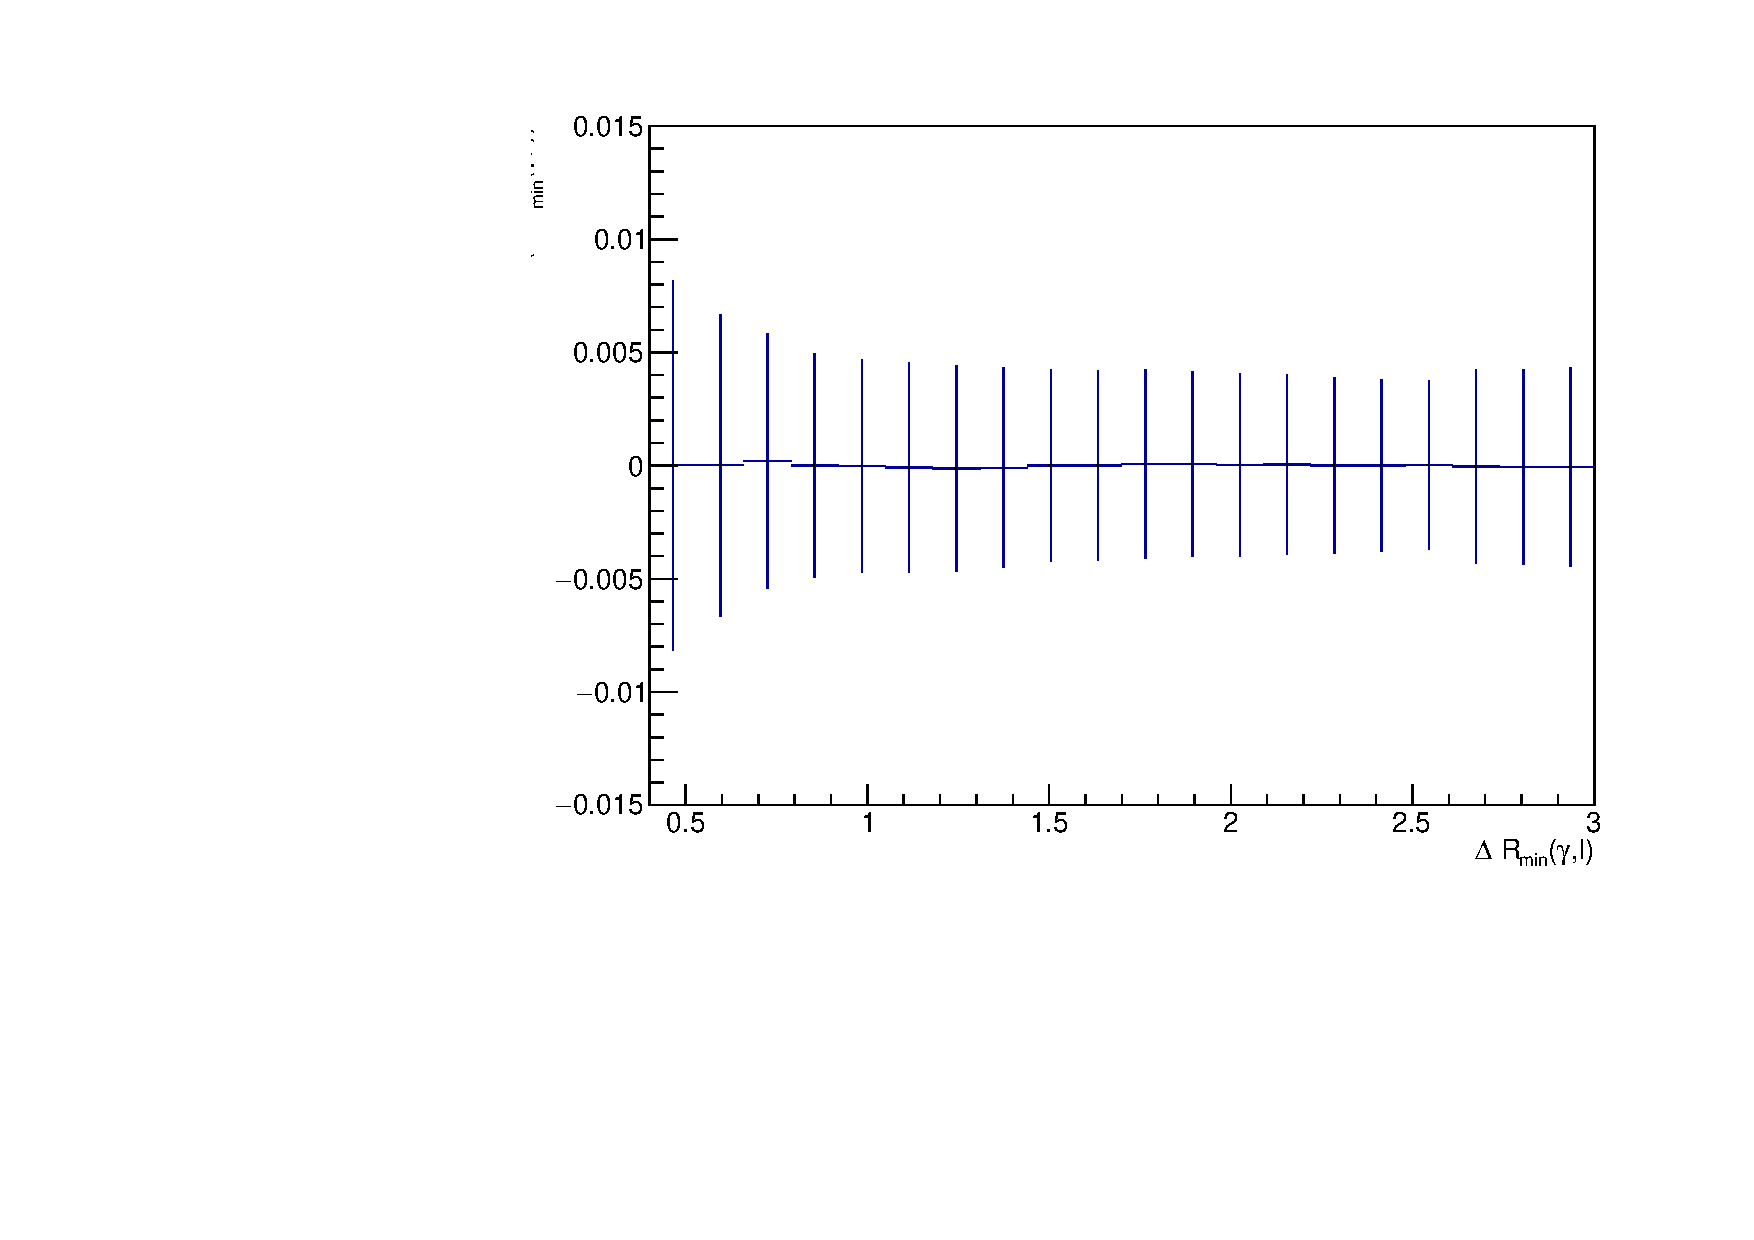
\includegraphics[width=0.4\textwidth]{figures/diff_xsec/binning_optimization/resolution/mean_stdDev_resolution_h2_ph_drphl_reco_part_full_weighted.pdf}} \\
    \subfloat[]{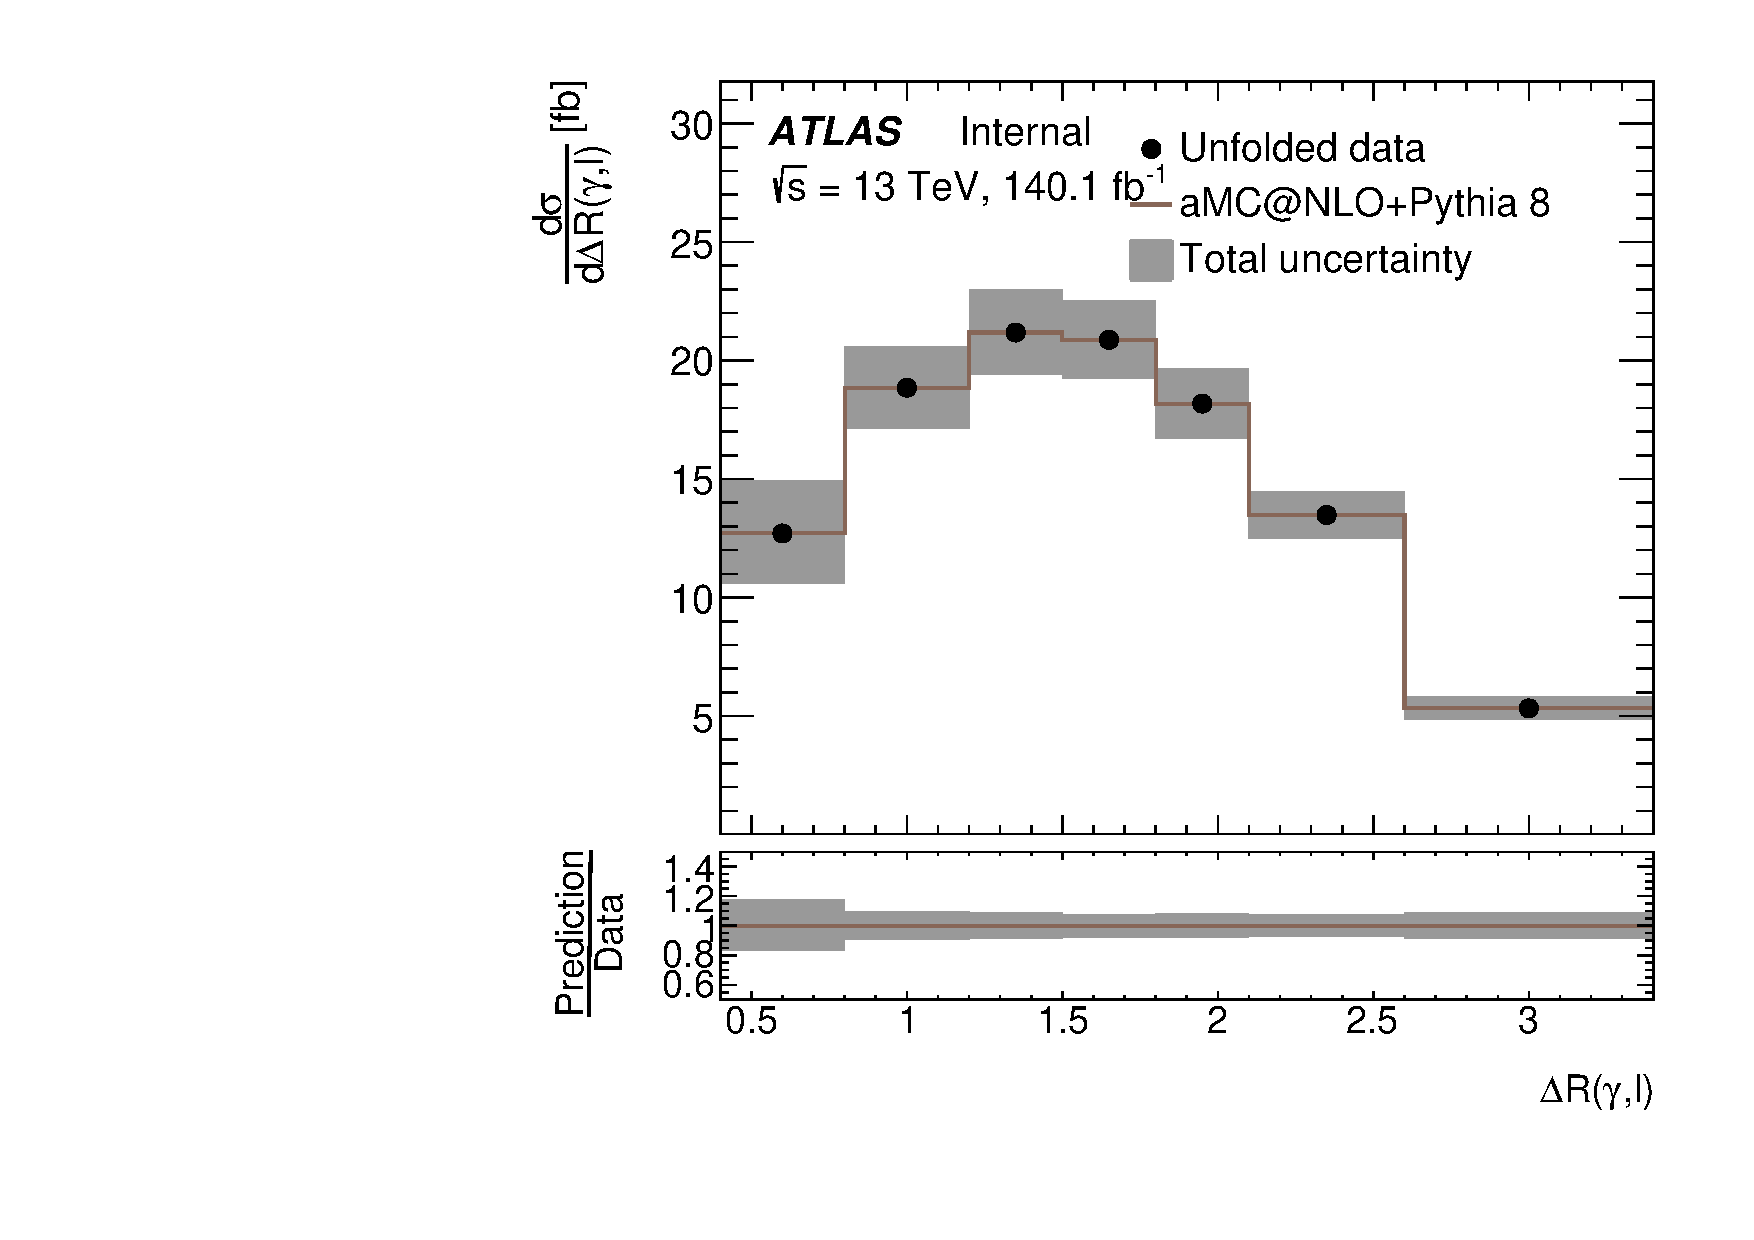
\includegraphics[width=0.23\textwidth]{figures/diff_xsec/binning_optimization/optimized_tty_prod/tty_min_drphl_UnfoldedData.pdf}}
    \hfill
    \subfloat[]{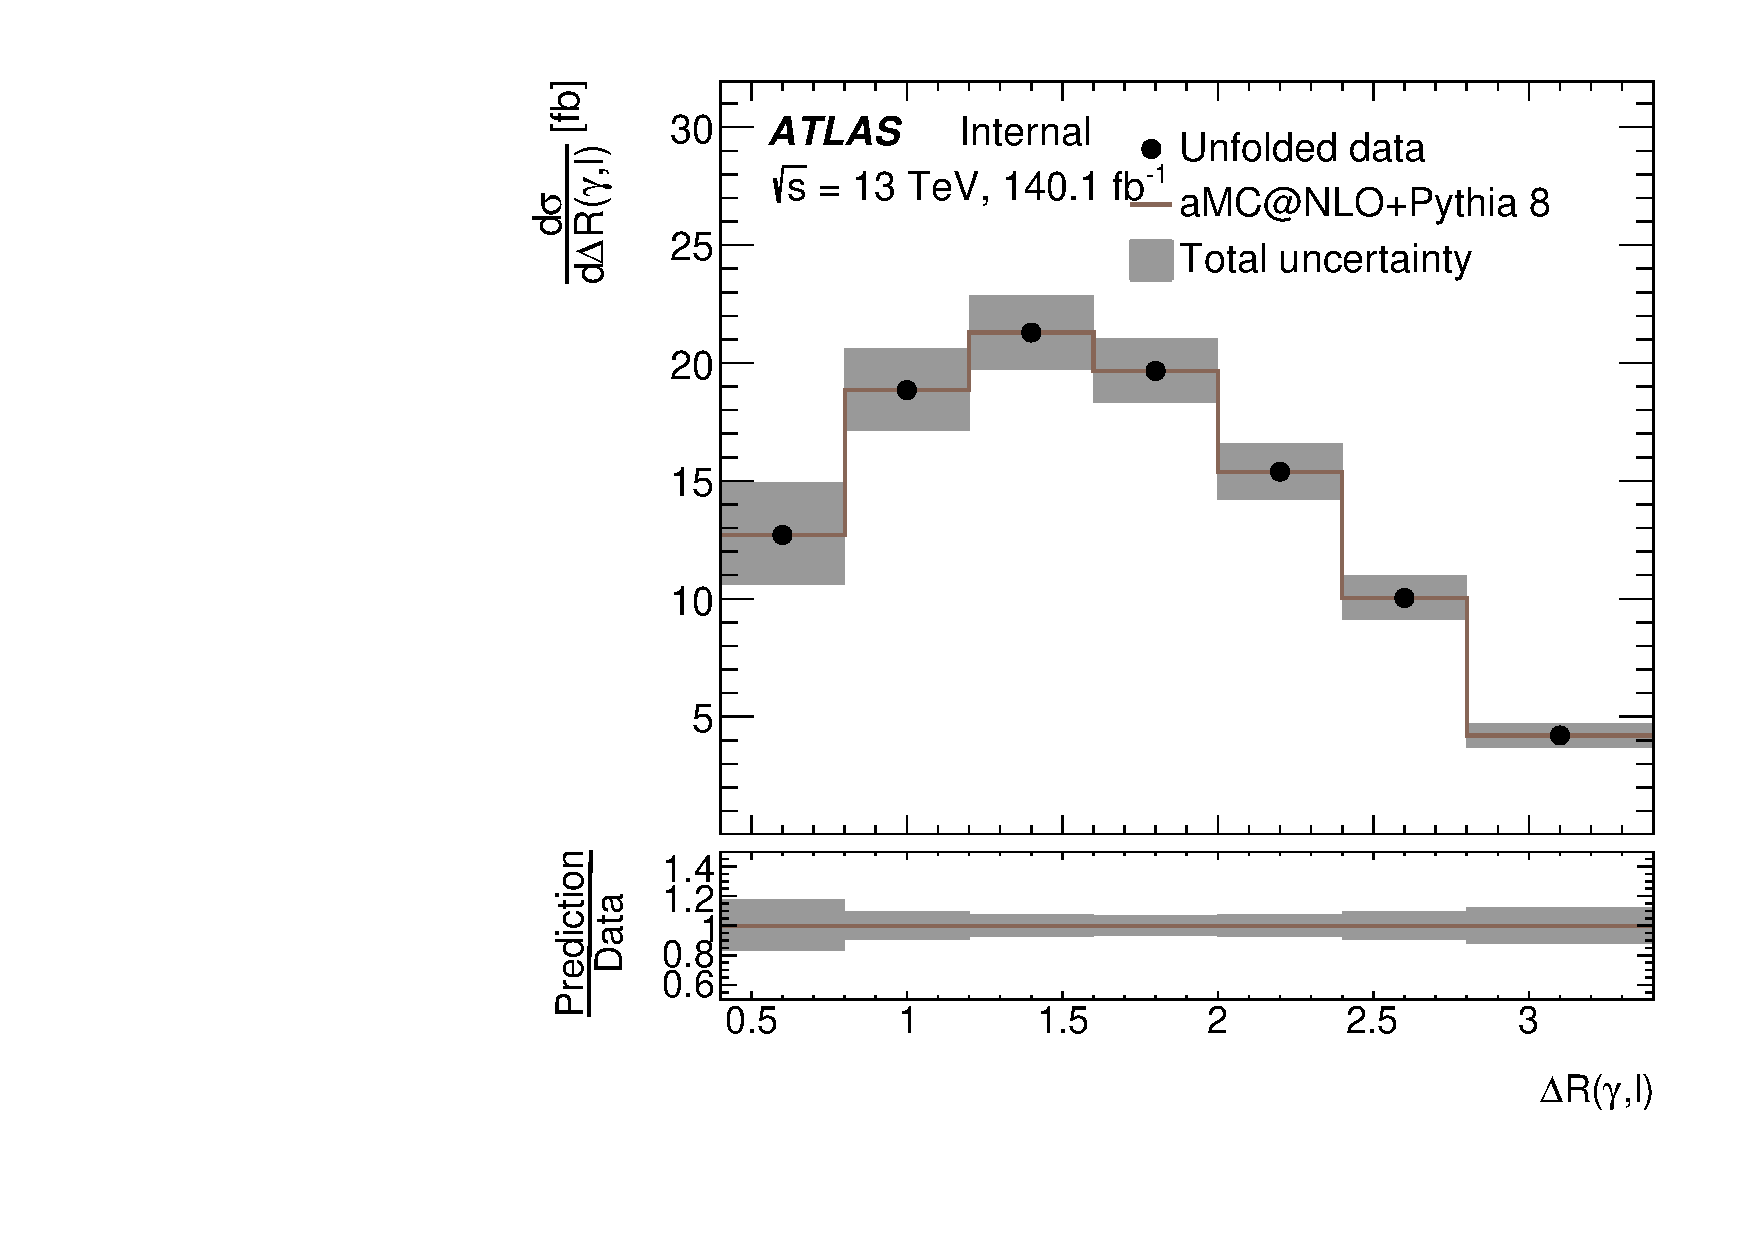
\includegraphics[width=0.23\textwidth]{figures/diff_xsec/binning_optimization/nominal_tty_prod/tty_min_drphl_UnfoldedData.pdf}}
    \hfill
    \subfloat[]{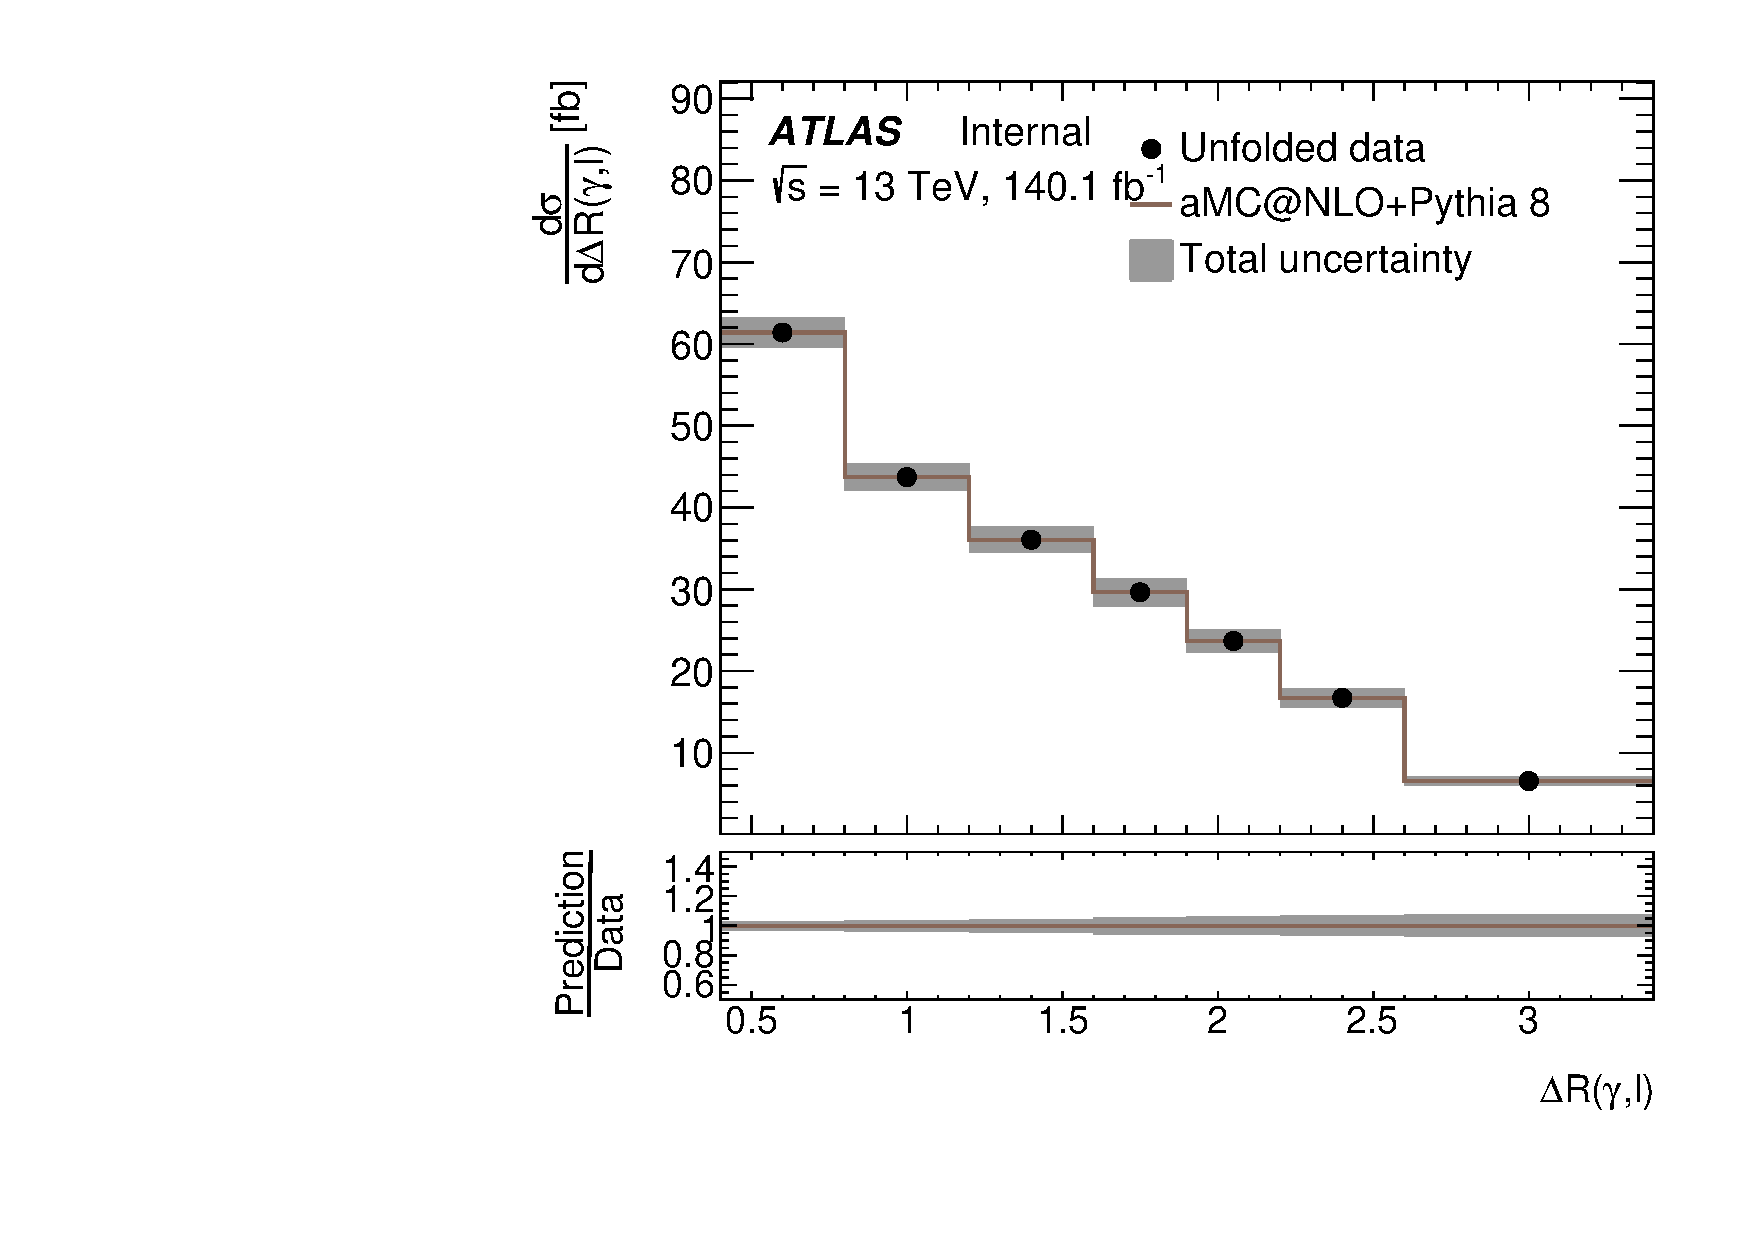
\includegraphics[width=0.23\textwidth]{figures/diff_xsec/binning_optimization/optimized_tty_incl/tty2l_dr_all_stat_UnfoldedData.pdf}}
    \hfill
    \subfloat[]{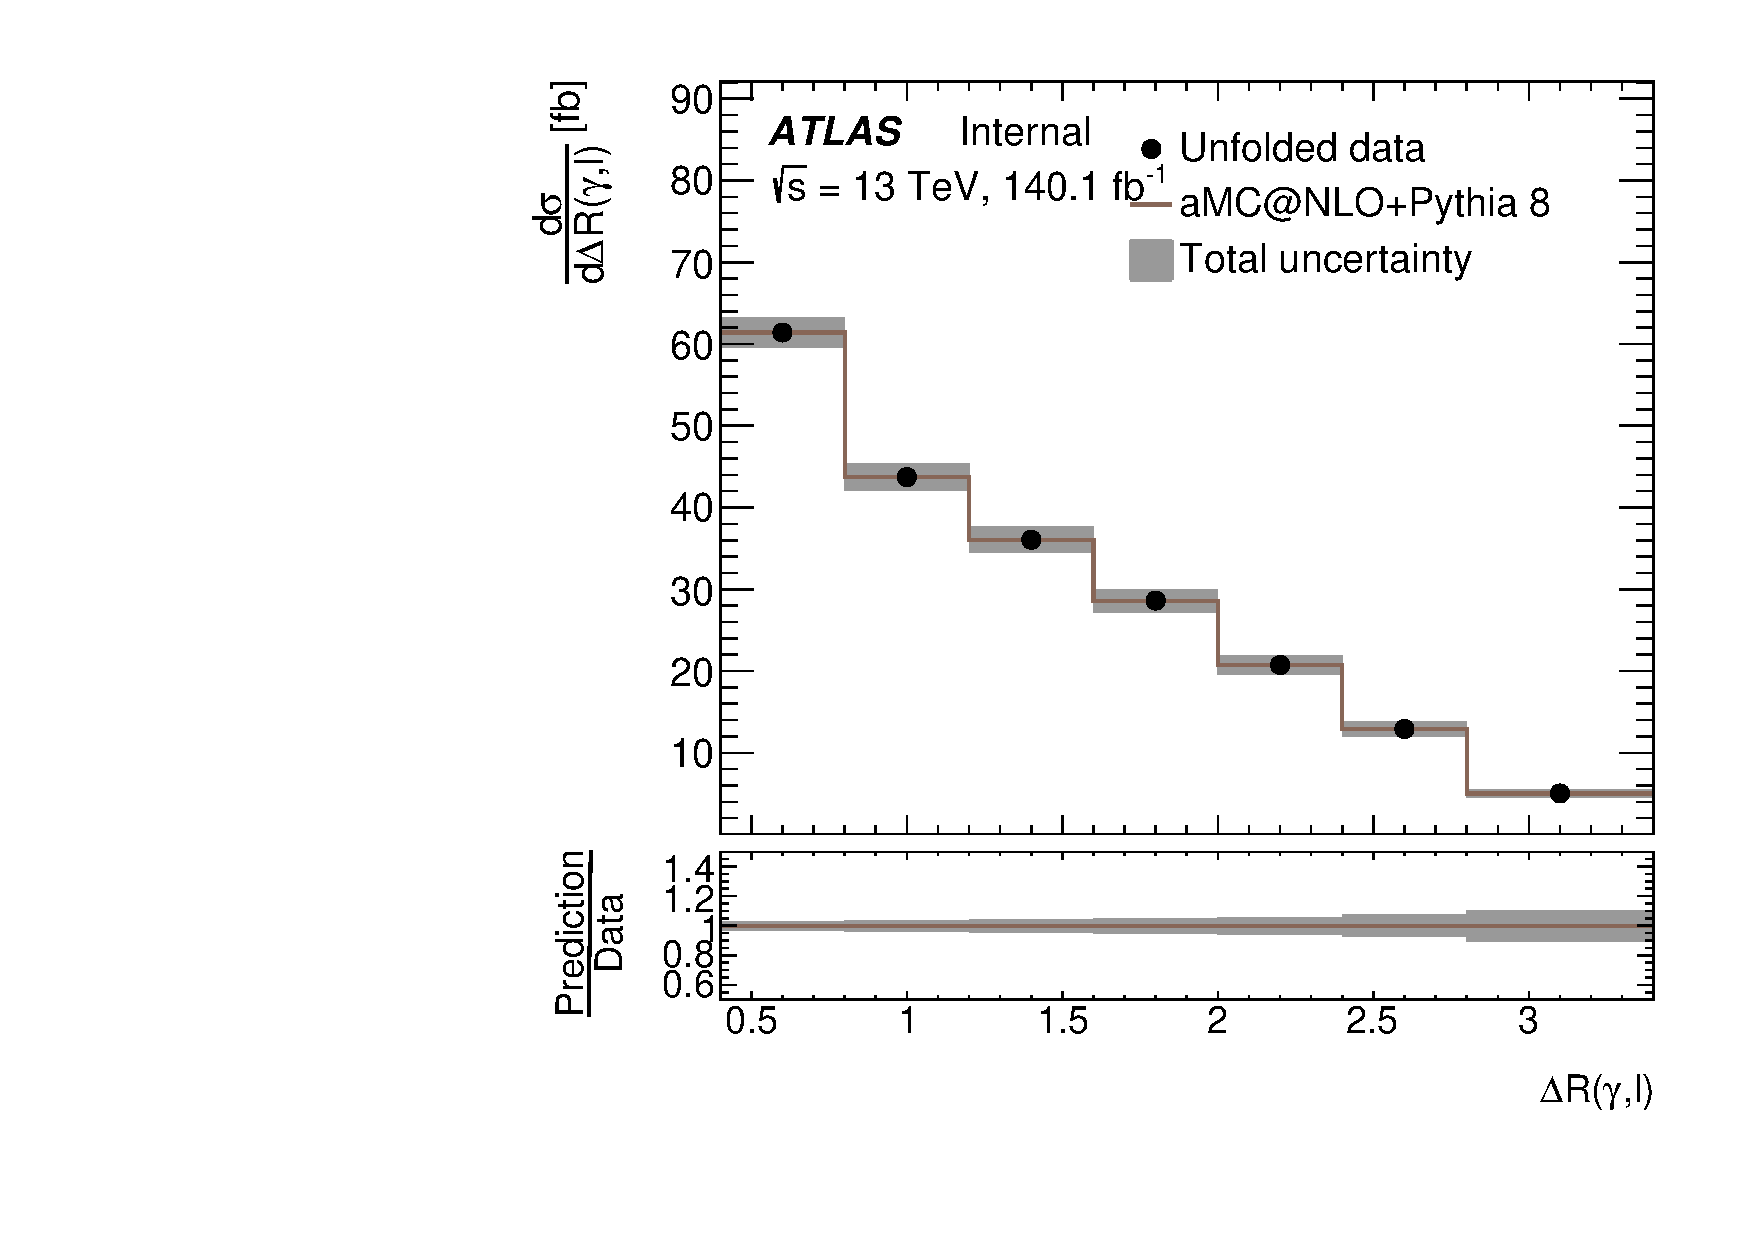
\includegraphics[width=0.23\textwidth]{figures/diff_xsec/binning_optimization/nominal_tty_incl/tty2l_dr_all_stat_UnfoldedData.pdf}}
    \hfill
    \subfloat[]{\includegraphics[width=0.23\textwidth]{figures/diff_xsec/binning_optimization/migrations/migration_tty_prod_06/migration_h2_ph_drphl_reco_part_full_weighted_SR1.pdf}}
    \hfill
    \subfloat[]{\includegraphics[width=0.23\textwidth]{figures/diff_xsec/binning_optimization/migrations/migration_tty_prod_nominal/migration_h2_ph_drphl_reco_part_full_weighted_SR1.pdf}}
    \hfill
    \subfloat[]{\includegraphics[width=0.23\textwidth]{figures/diff_xsec/binning_optimization/migrations/migration_tty_incl_06/migration_h2_ph_drphl_reco_part_full_weighted_SR1.pdf}}
    \hfill
    \subfloat[]{\includegraphics[width=0.23\textwidth]{figures/diff_xsec/binning_optimization/migrations/migration_tty_incl_nominal/migration_h2_ph_drphl_reco_part_full_weighted_SR1.pdf}}
    \hfill


    \caption{(a) Resolution of the photon $\Delta R_{min}(\gamma,l)$ observable is represented by the error bars. The y-axis
    is the mean of (reconstructed photon $\Delta R_{min}(\gamma,l)$ - truth photon $\Delta R_{min}(\gamma,l)$) in GeV and the error bars represent
    one standard deviation around that mean.
    Unfolded results with the tested binning (b) and final
    binning (c) for \tty(prod) measurement and unfolded results with the tested
    (d) and final (e) binning for \tty(total) measurement, The error bar in (b),
    (c), (d), (e) represents statistical uncertainty only.
    The error bar in (b), (c), (d), (e) represents statistical uncertainty only.
    Plots (f)- (i) represents the migration matrix in the SR for above cases.}
\end{figure}
\FloatBarrier

%%%% dEta(ll) %%%
\begin{figure}[ht]
    \centering
    \subfloat[]{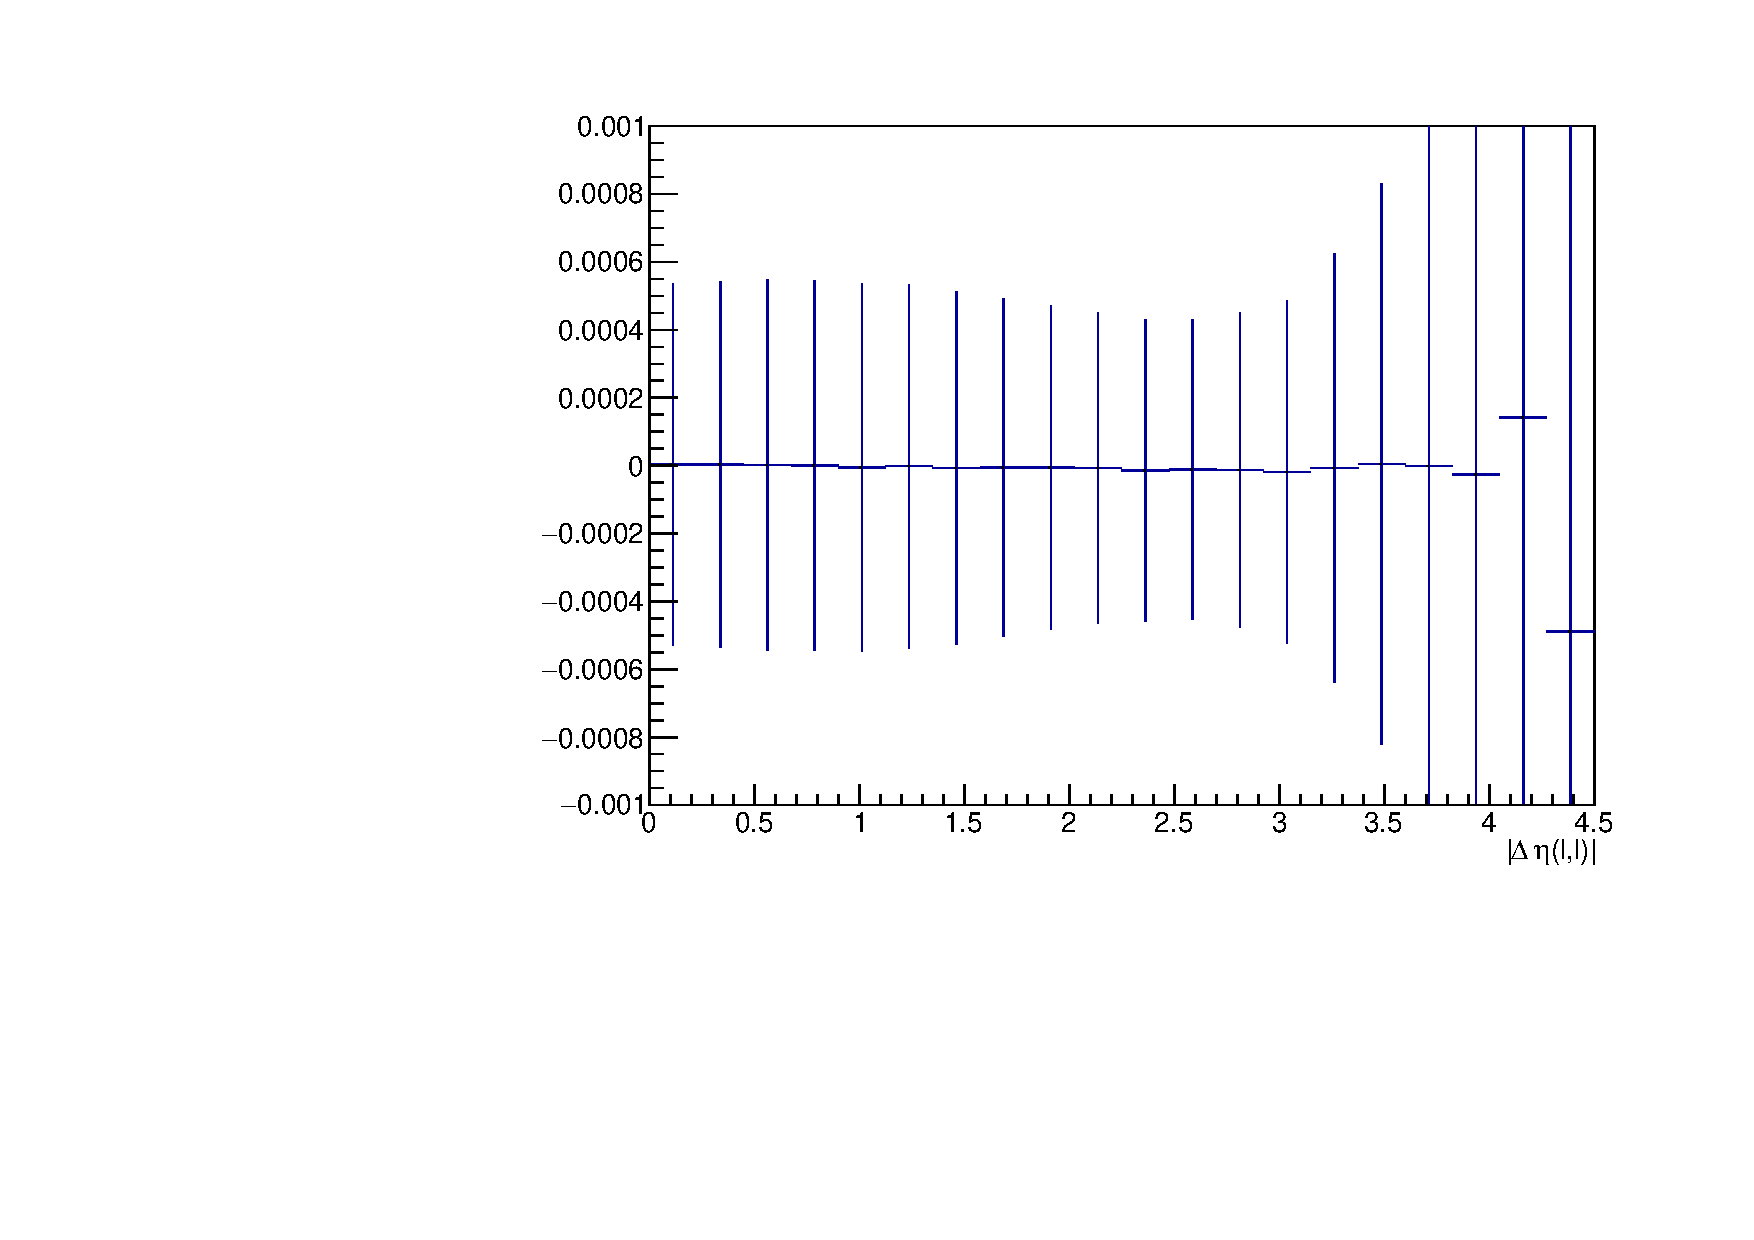
\includegraphics[width=0.4\textwidth]{figures/diff_xsec/binning_optimization/resolution/mean_stdDev_resolution_h2_dEtall_reco_part_full_weighted.pdf}} \\
    \subfloat[]{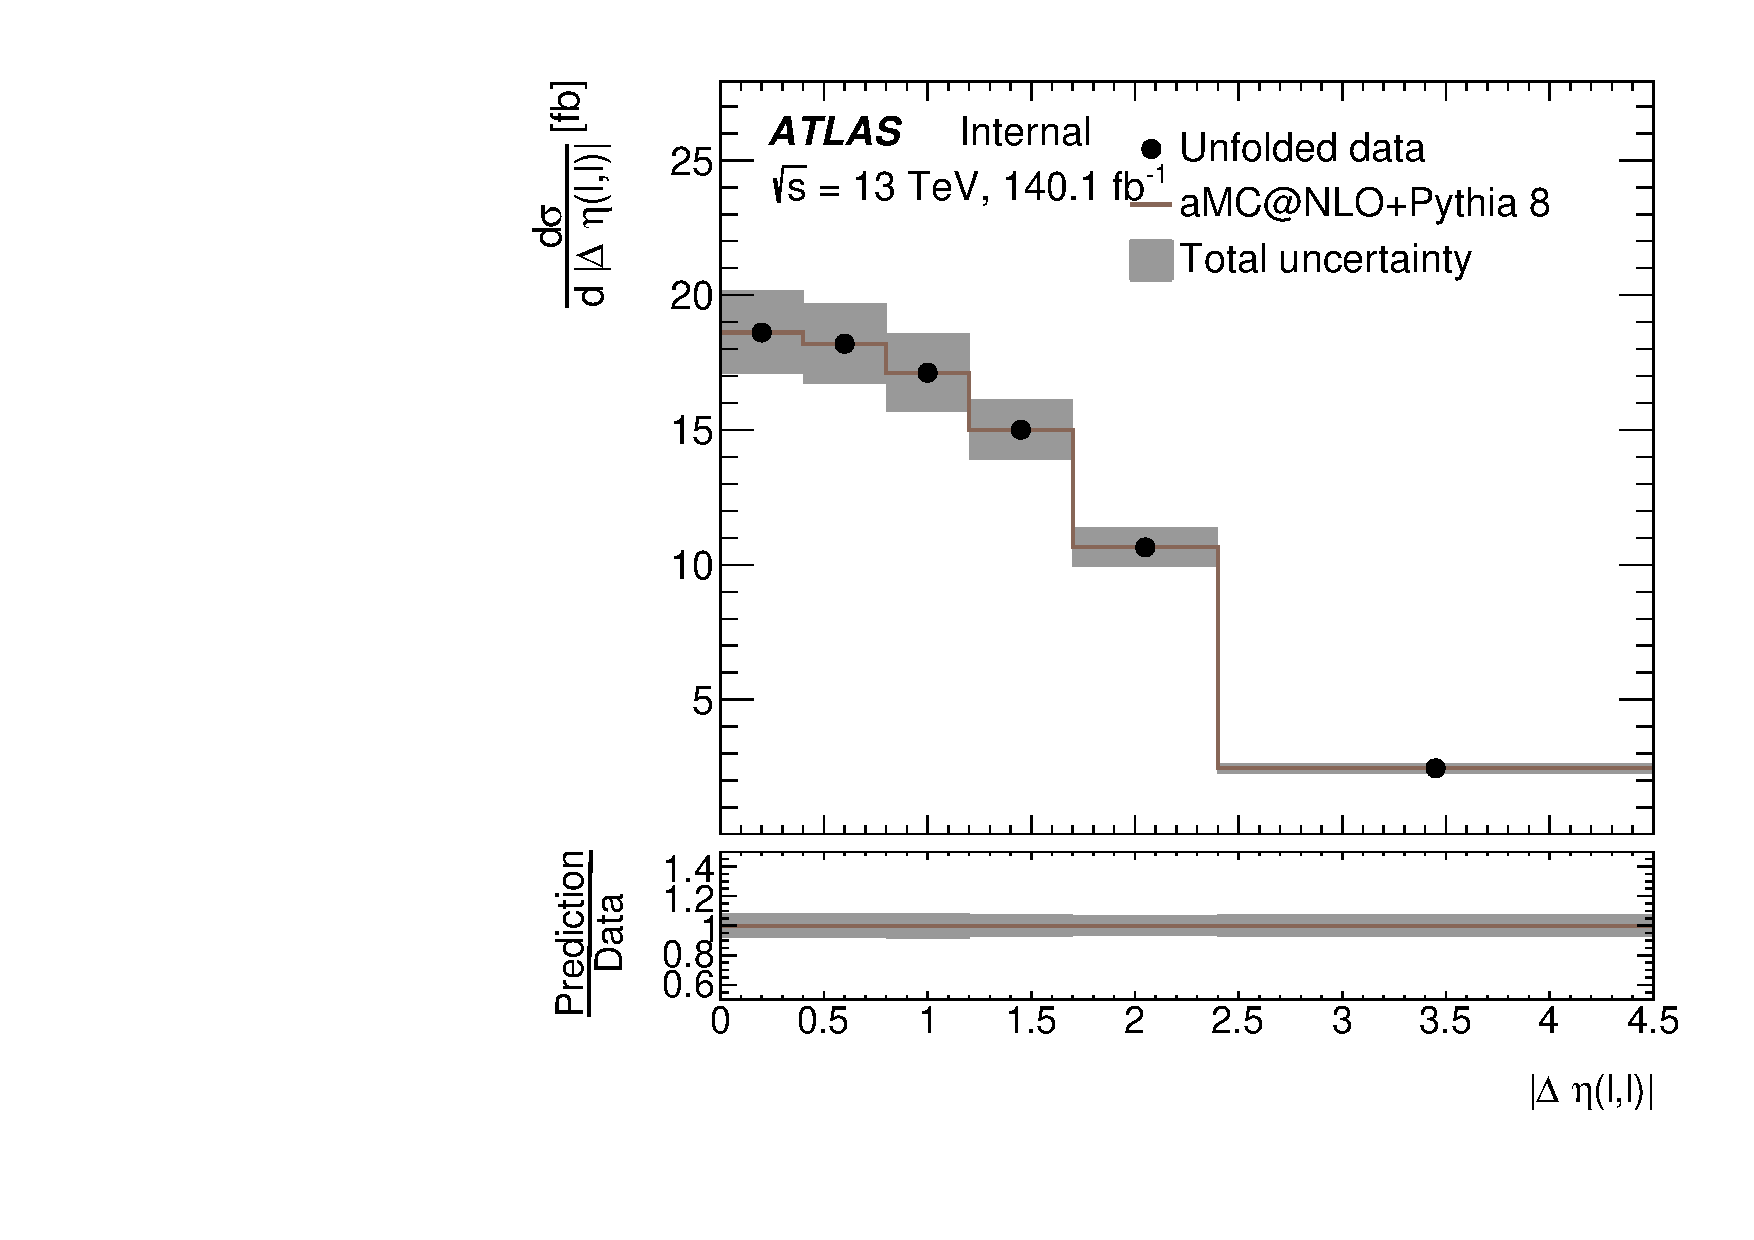
\includegraphics[width=0.23\textwidth]{figures/diff_xsec/binning_optimization/optimized_tty_prod/tty_dEtall_UnfoldedData.pdf}}
    \hfill
    \subfloat[]{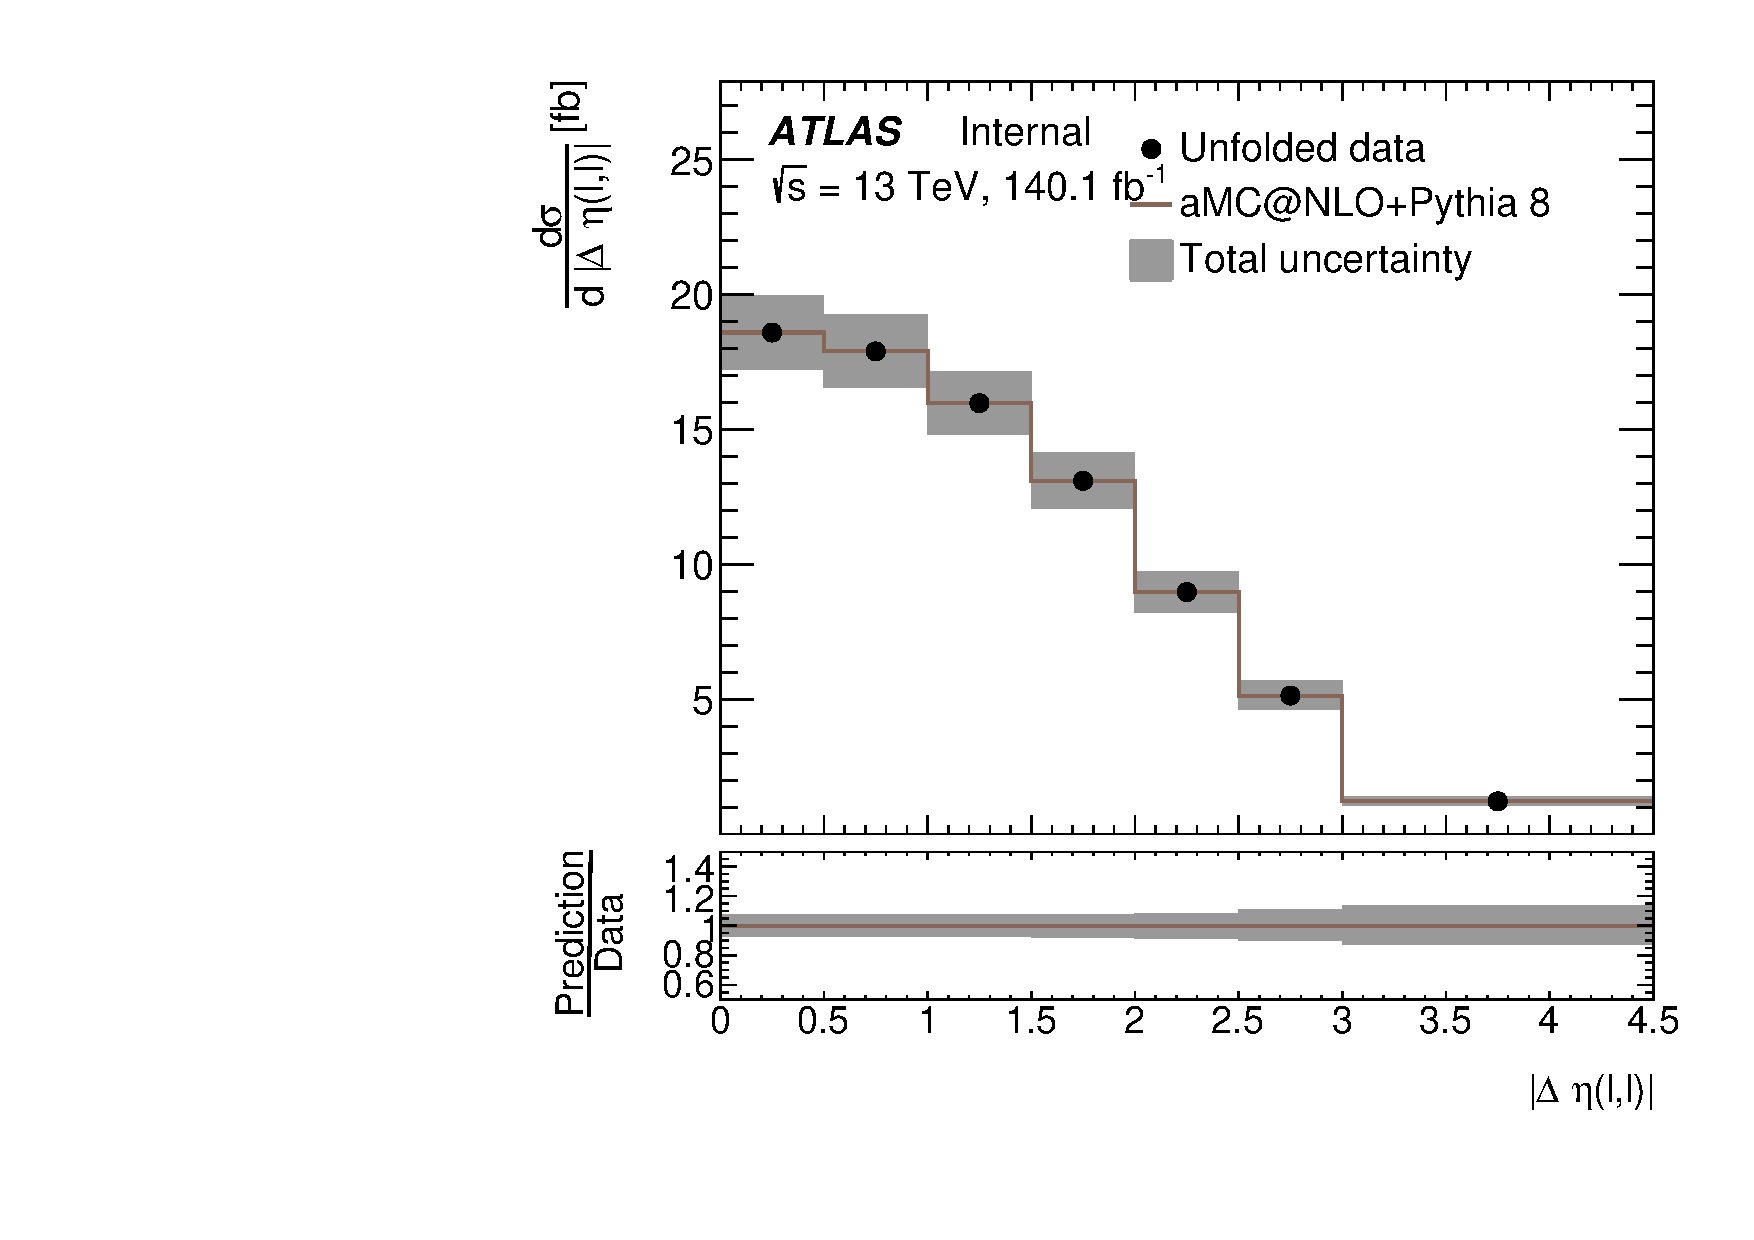
\includegraphics[width=0.23\textwidth]{figures/diff_xsec/binning_optimization/nominal_tty_prod/tty_dEtall_UnfoldedData.pdf}}
    \hfill
    \subfloat[]{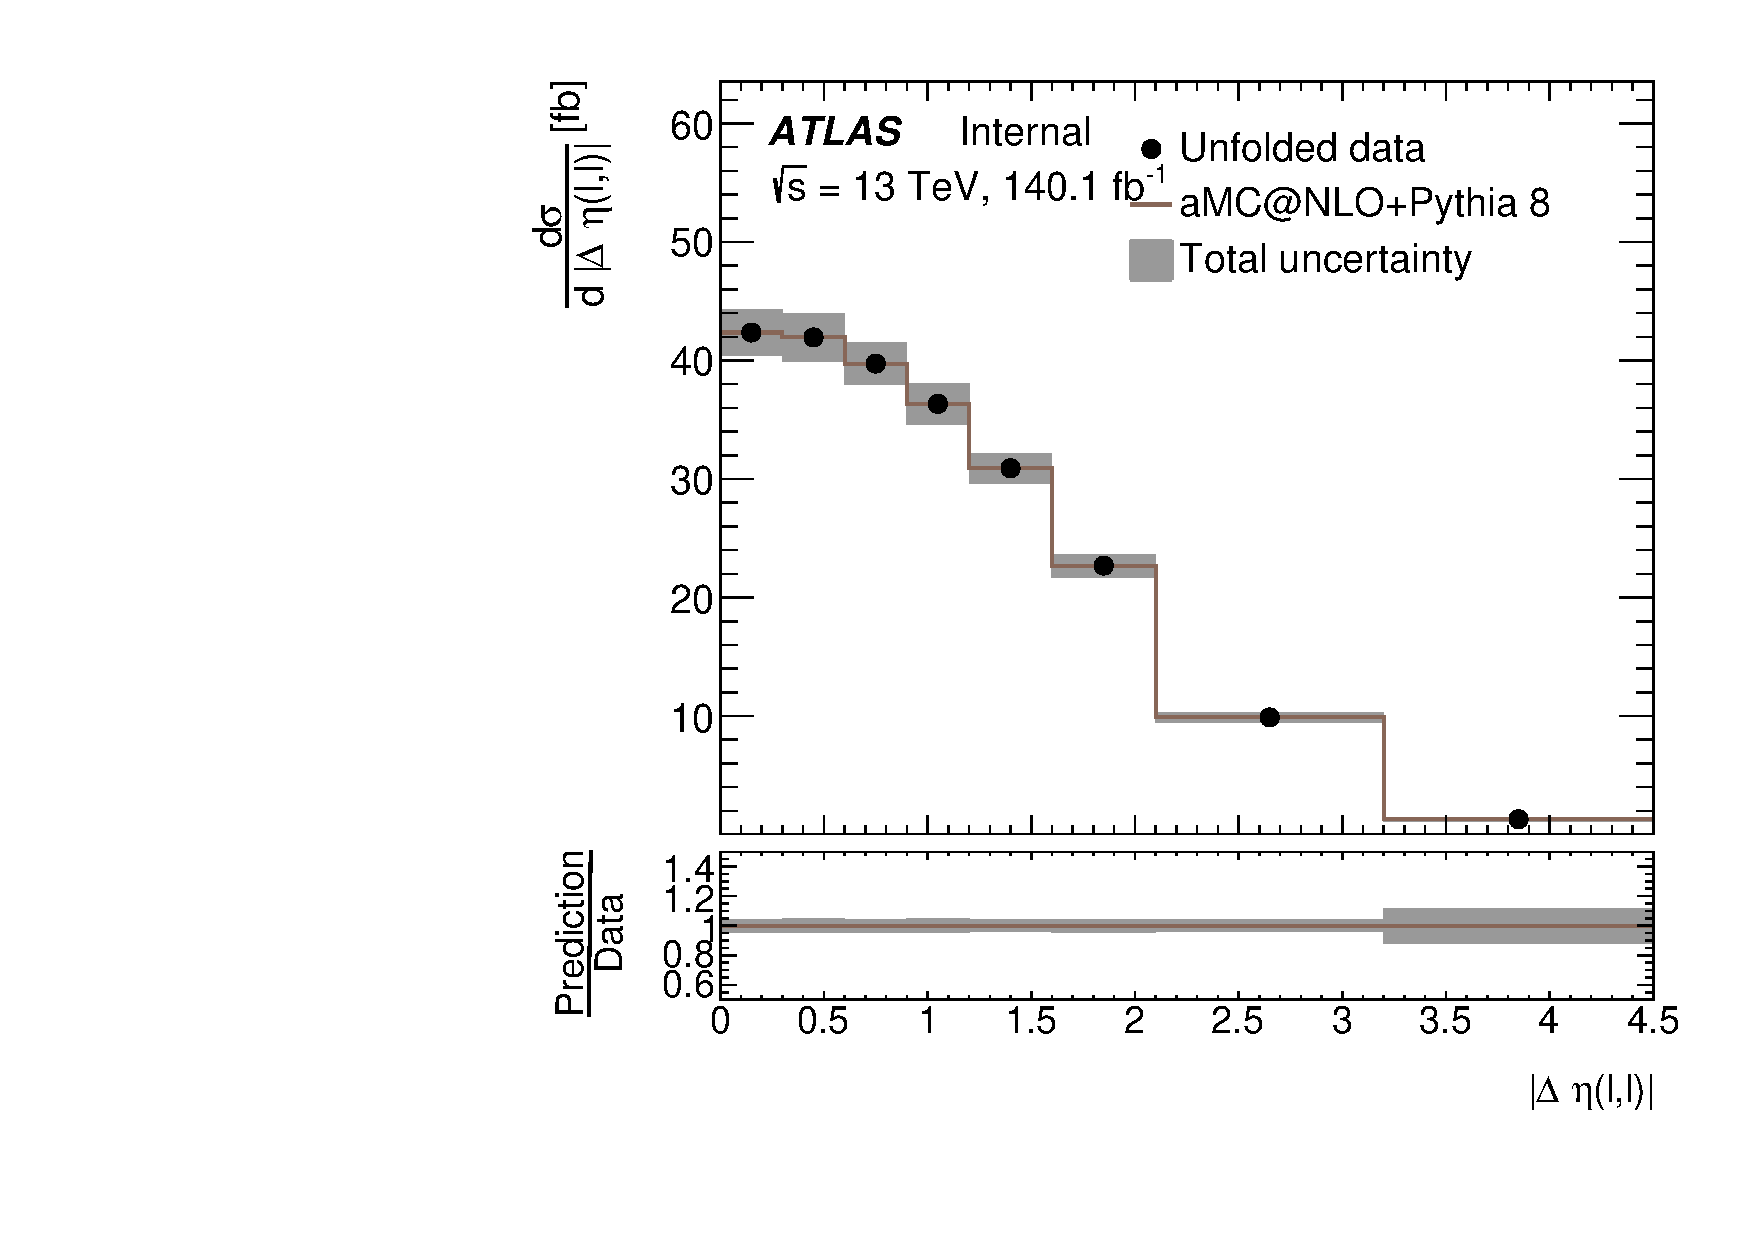
\includegraphics[width=0.23\textwidth]{figures/diff_xsec/binning_optimization/optimized_tty_incl/tty2l_dEtall_all_stat_UnfoldedData.pdf}}
    \hfill
    \subfloat[]{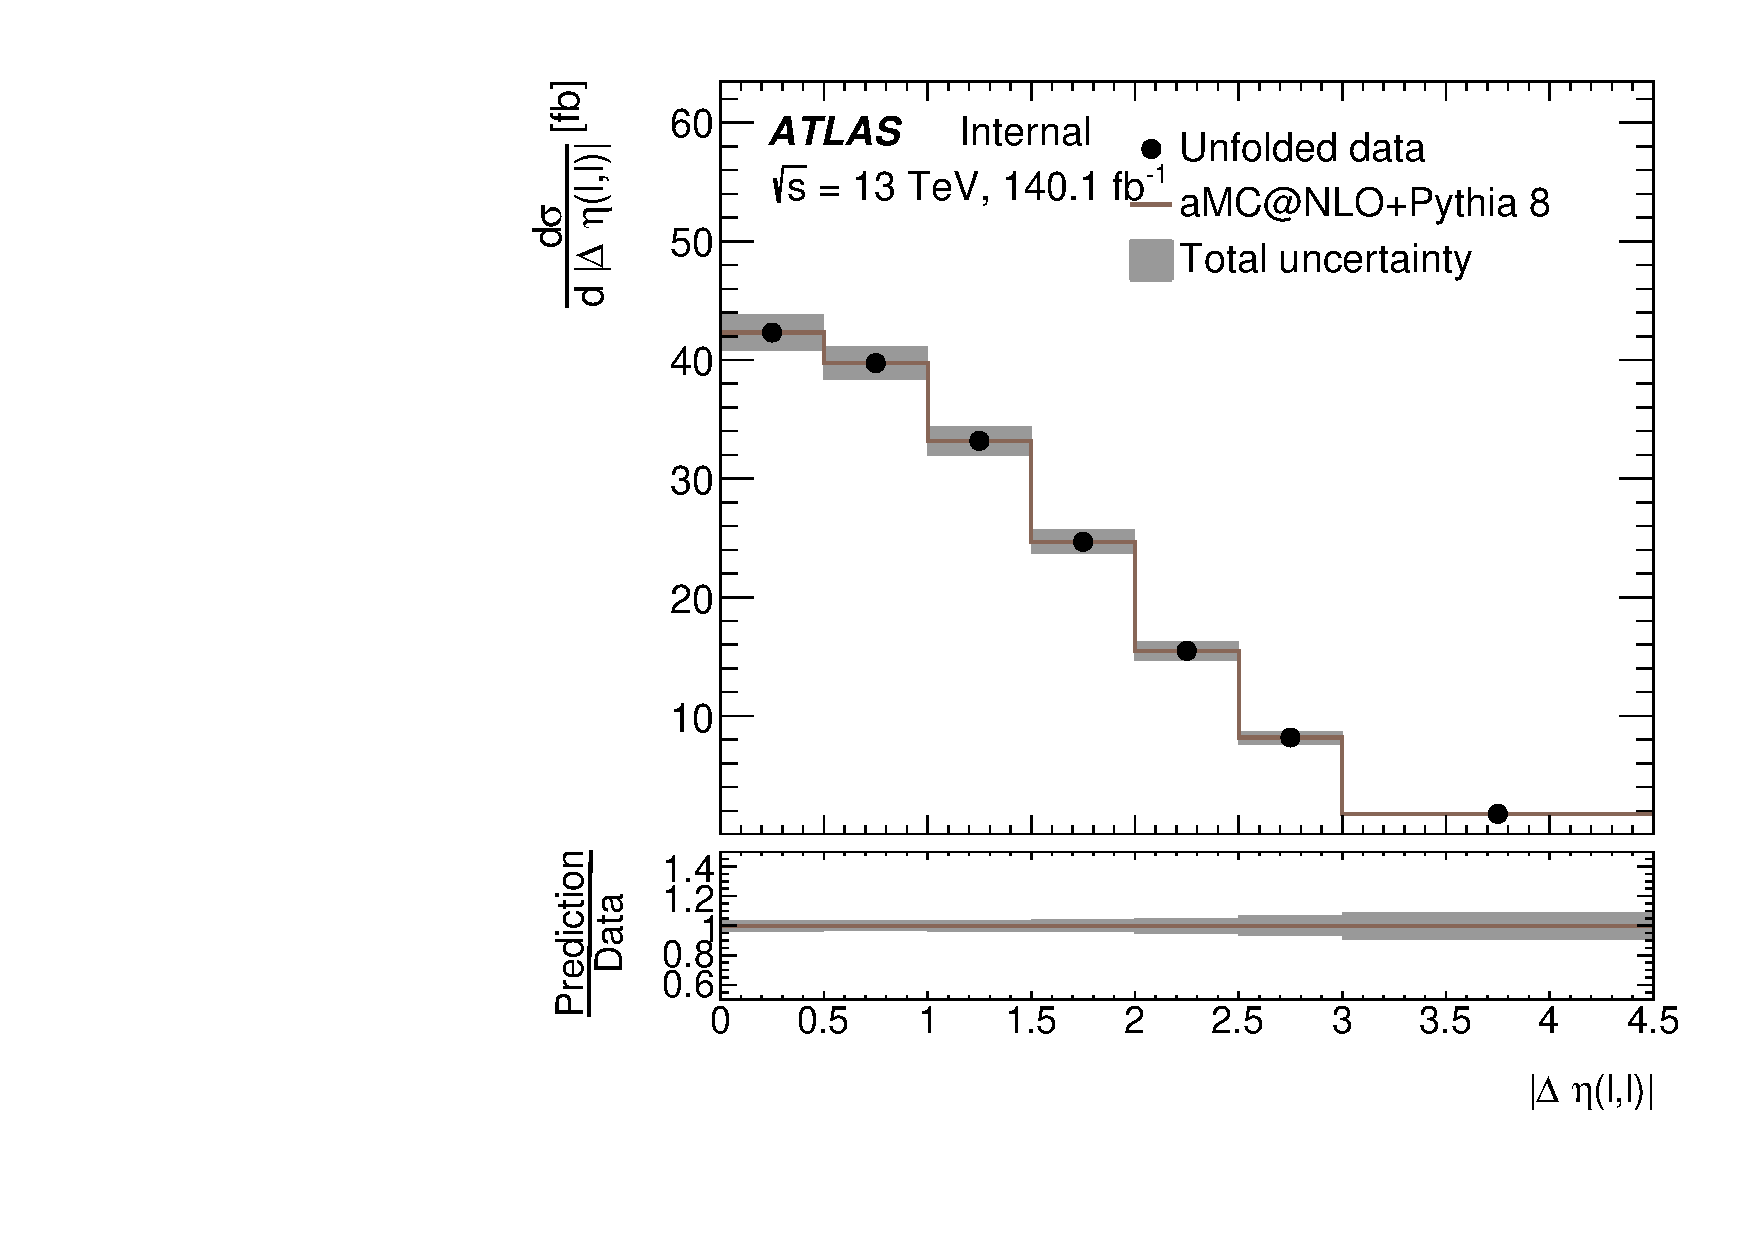
\includegraphics[width=0.23\textwidth]{figures/diff_xsec/binning_optimization/nominal_tty_incl/tty2l_dEtall_all_stat_UnfoldedData.pdf}}
    \hfill
    \subfloat[]{\includegraphics[width=0.23\textwidth]{figures/diff_xsec/binning_optimization/migrations/migration_tty_prod_06/migration_h2_dEtall_reco_part_full_weighted_SR1.pdf}}
    \hfill
    \subfloat[]{\includegraphics[width=0.23\textwidth]{figures/diff_xsec/binning_optimization/migrations/migration_tty_prod_nominal/migration_h2_dEtall_reco_part_full_weighted_SR1.pdf}}
    \hfill
    \subfloat[]{\includegraphics[width=0.23\textwidth]{figures/diff_xsec/binning_optimization/migrations/migration_tty_incl_06/migration_h2_dEtall_reco_part_full_weighted_SR1.pdf}}
    \hfill
    \subfloat[]{\includegraphics[width=0.23\textwidth]{figures/diff_xsec/binning_optimization/migrations/migration_tty_incl_nominal/migration_h2_dEtall_reco_part_full_weighted_SR1.pdf}}
    \hfill

    \caption{(a) Resolution of the photon $|\Delta \eta(l,l)|$ observable is represented by the error bars. The y-axis
    is the mean of (reconstructed photon $|\Delta \eta(l,l)|$ - truth photon $|\Delta \eta(l,l)|$) in GeV and the error bars represent
    one standard deviation around that mean.
    Unfolded results with the tested binning (b) and final
    binning (c) for \tty(prod) measurement and unfolded results with the tested
    (d) and final (e) binning for \tty(total) measurement, The error bar in (b),
    (c), (d), (e) represents statistical uncertainty only.
    The error bar in (b), (c), (d), (e) represents statistical uncertainty only.
    Plots (f)- (i) represents the migration matrix in the SR for above cases.}

\end{figure}
\FloatBarrier

%%%% dPhi(ll) %%%
\begin{figure}[ht]
    \centering
    \subfloat[]{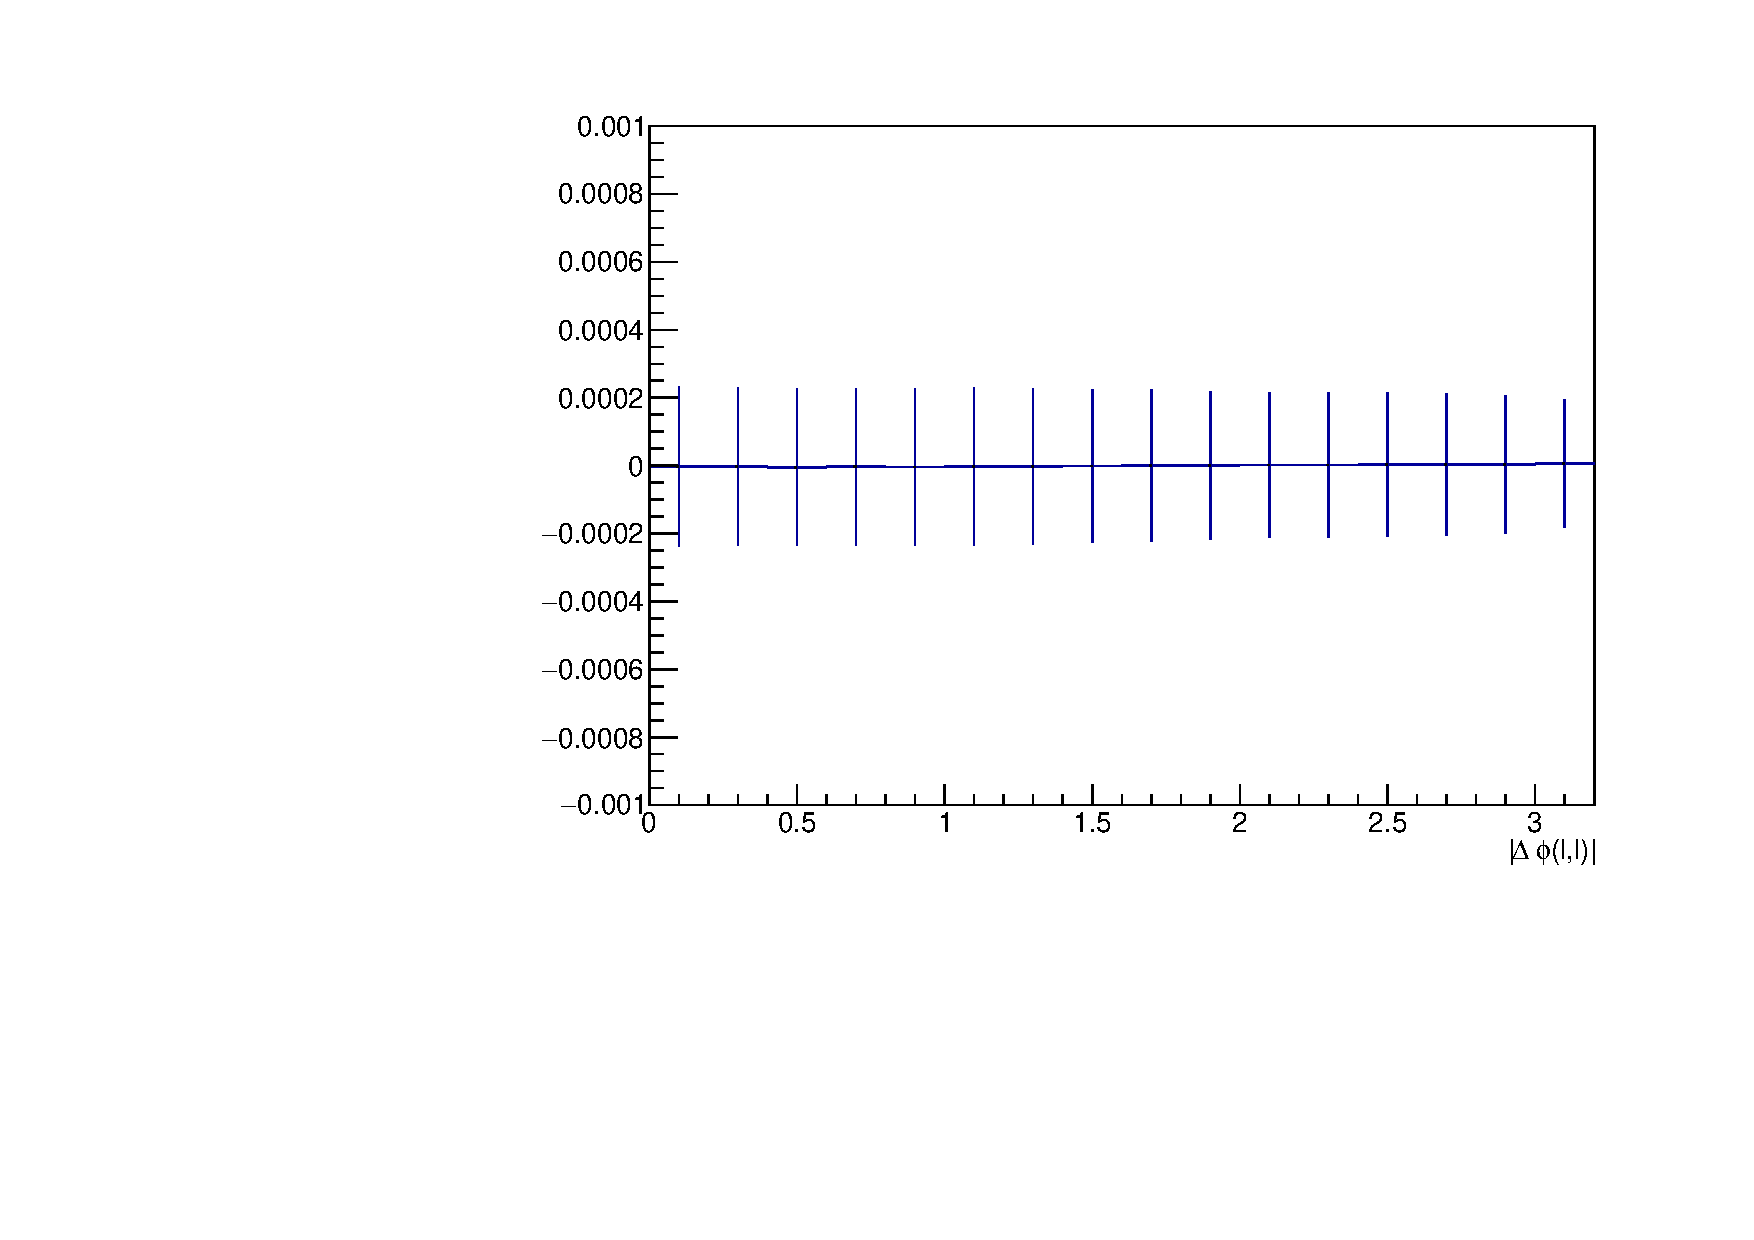
\includegraphics[width=0.4\textwidth]{figures/diff_xsec/binning_optimization/resolution/mean_stdDev_resolution_h2_dPhill_reco_part_full_weighted.pdf}} \\
    \subfloat[]{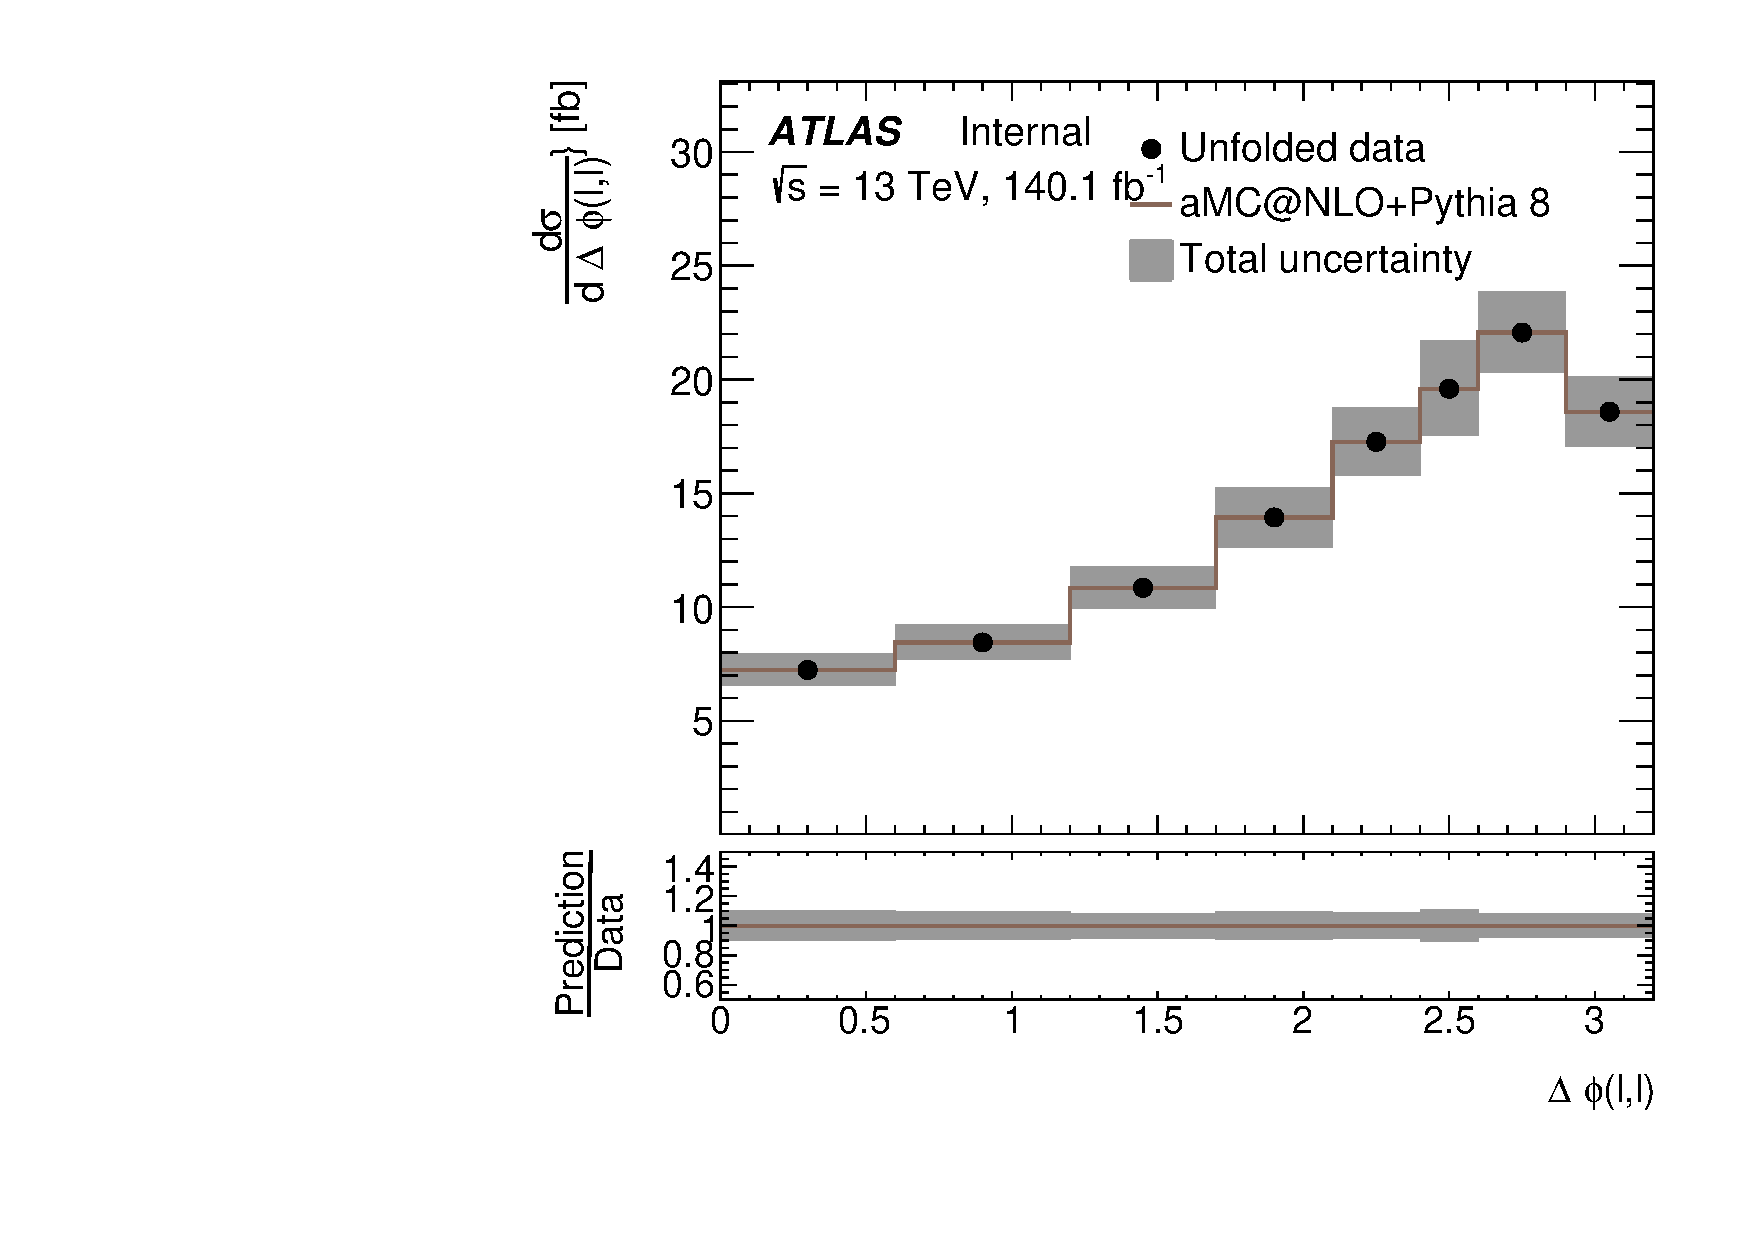
\includegraphics[width=0.23\textwidth]{figures/diff_xsec/binning_optimization/optimized_tty_prod/tty_dPhill_UnfoldedData.pdf}}
    \hfill
    \subfloat[]{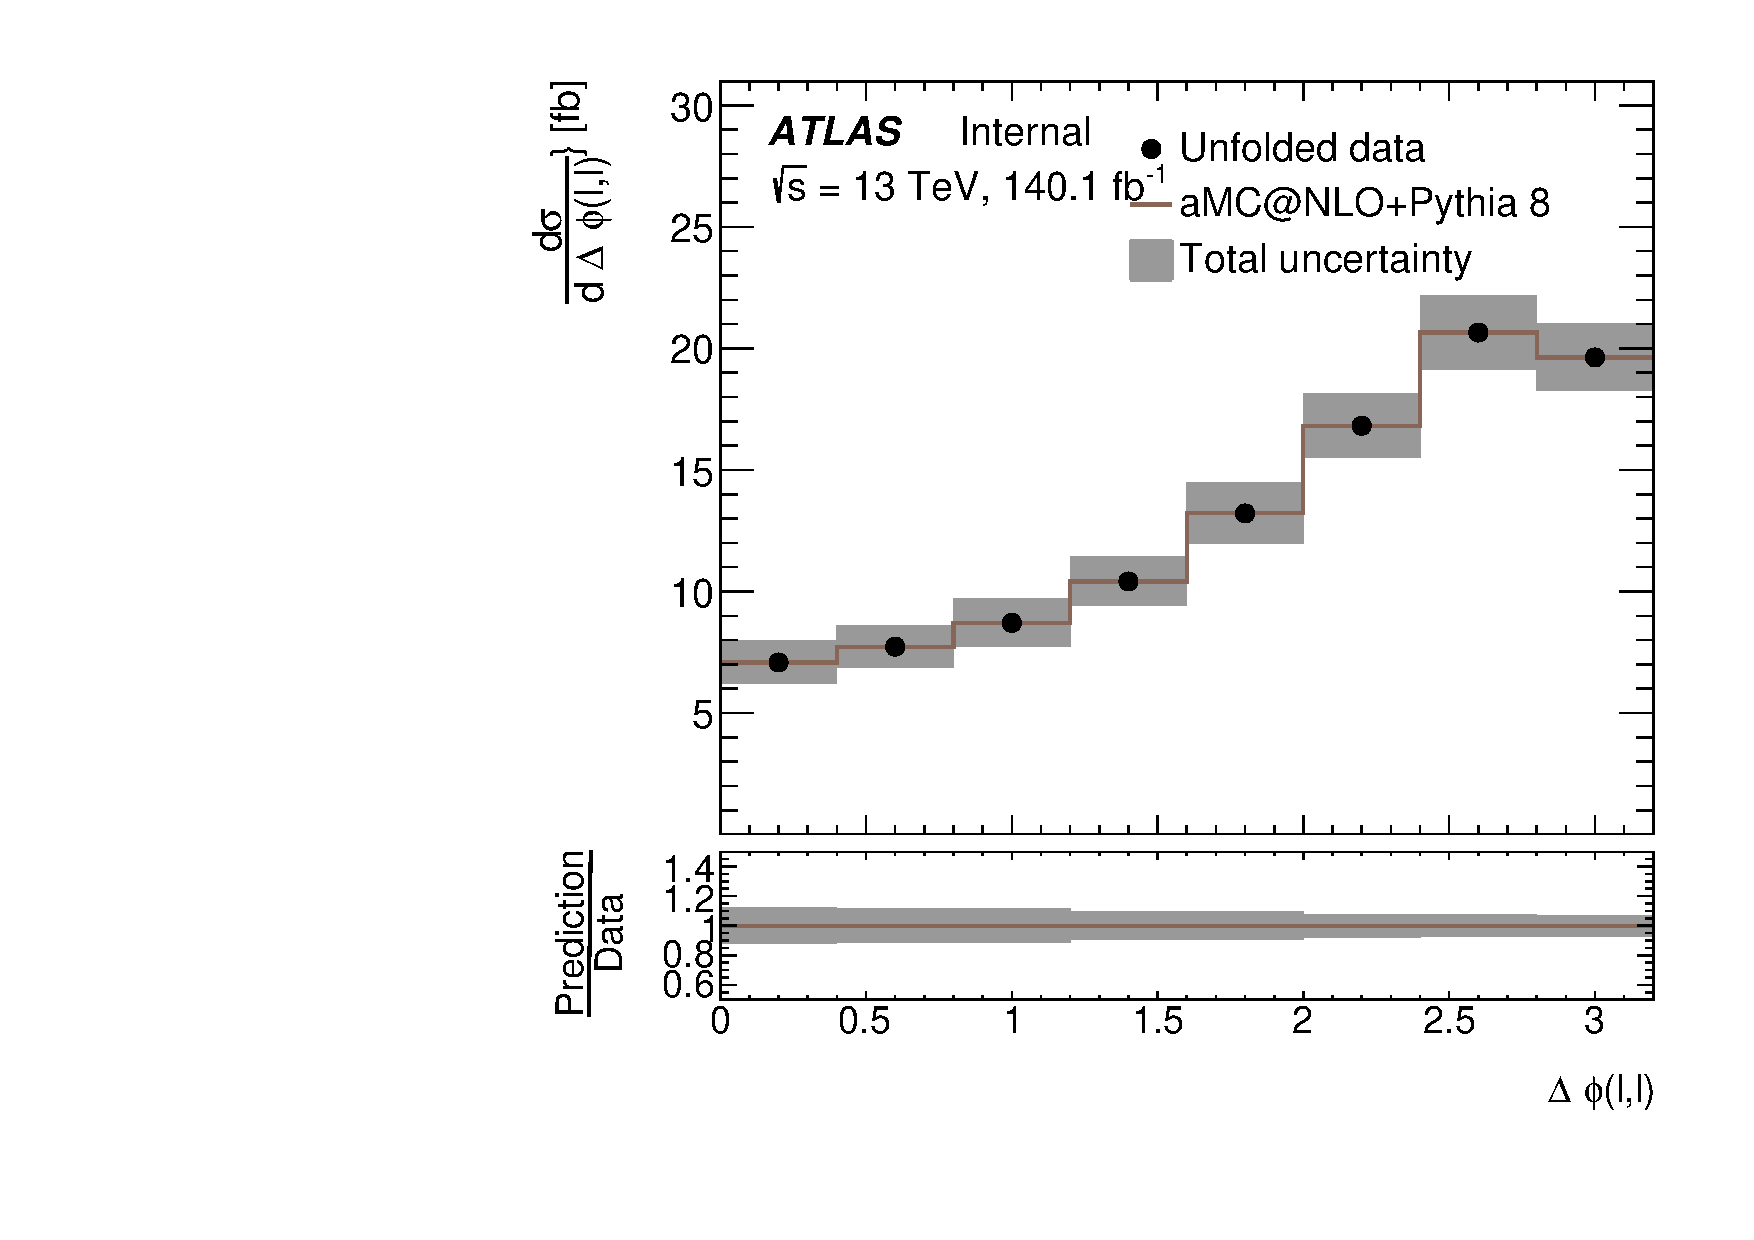
\includegraphics[width=0.23\textwidth]{figures/diff_xsec/binning_optimization/nominal_tty_prod/tty_dPhill_UnfoldedData.pdf}}
    \hfill
    \subfloat[]{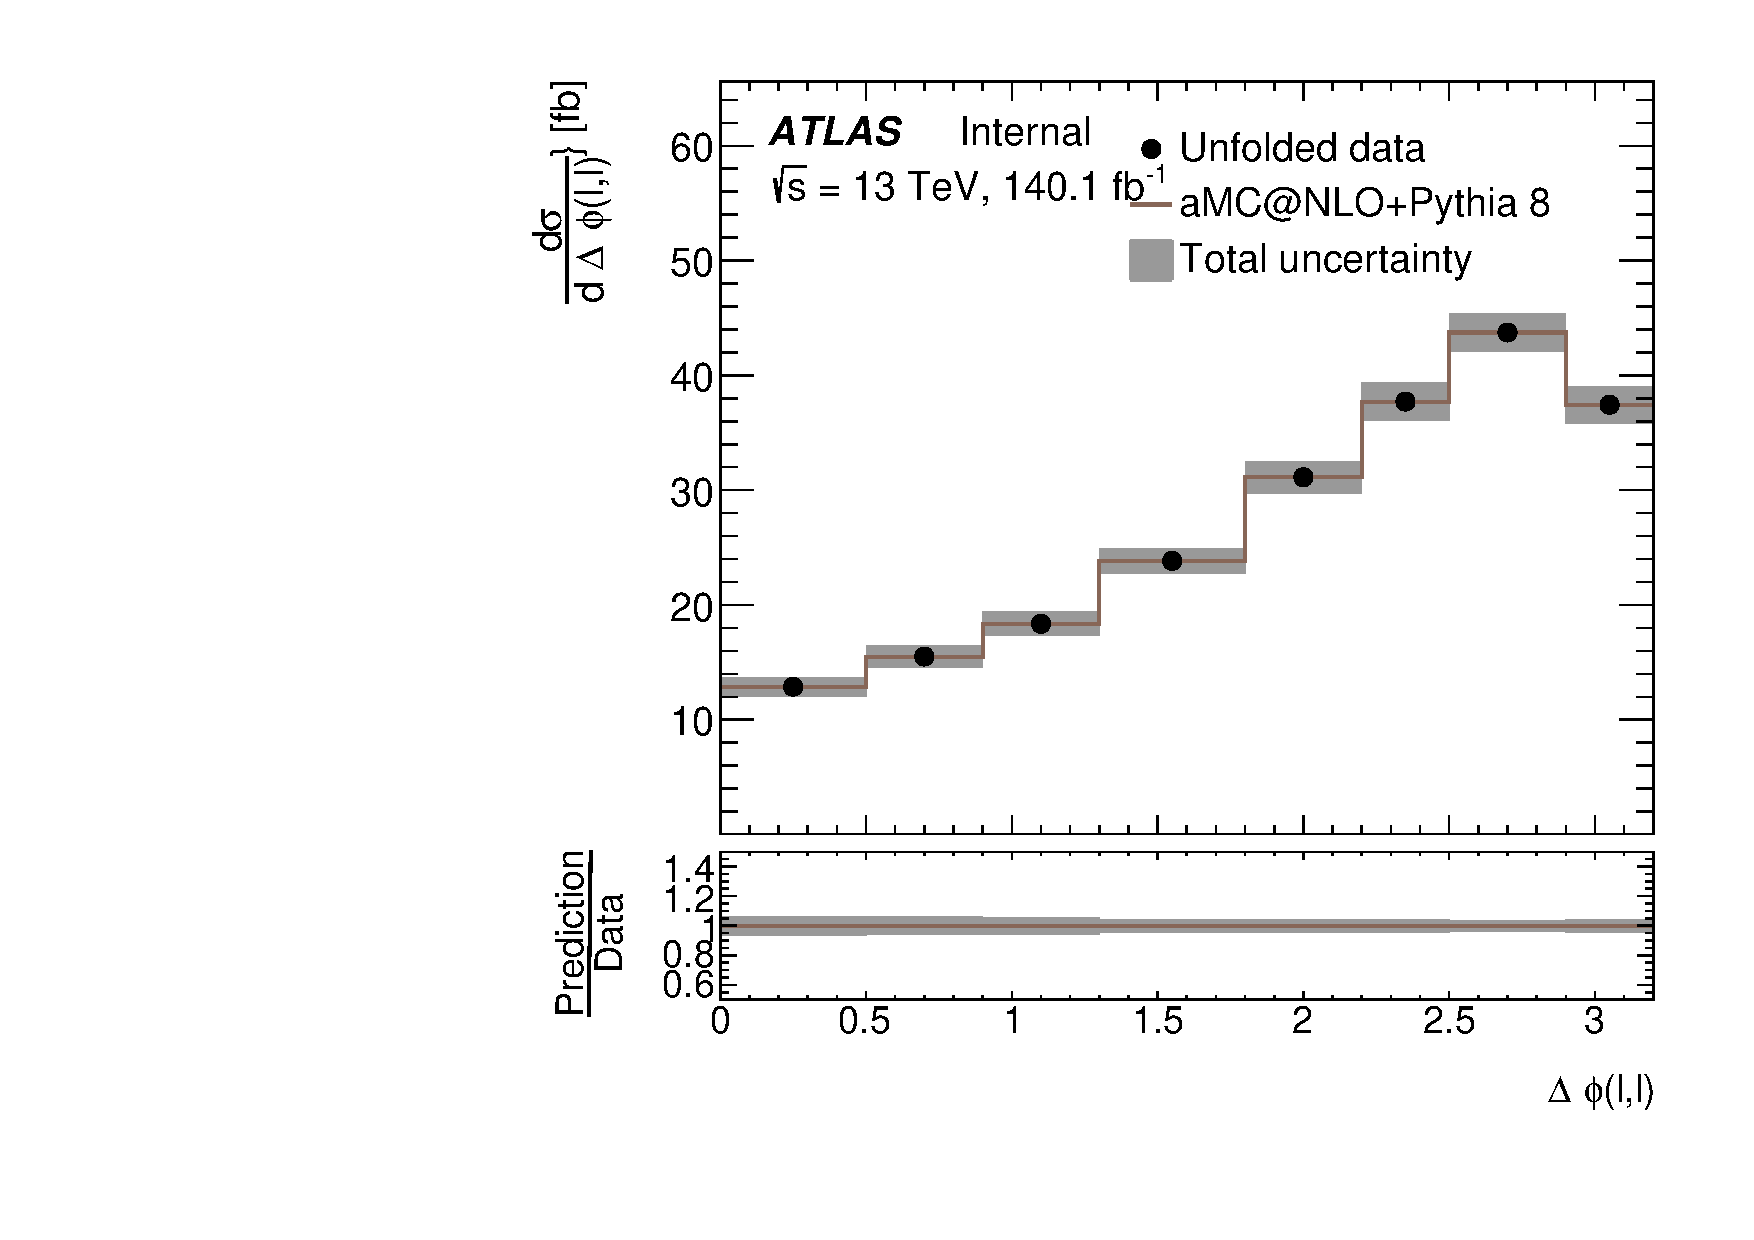
\includegraphics[width=0.23\textwidth]{figures/diff_xsec/binning_optimization/optimized_tty_incl/tty2l_dPhill_all_stat_UnfoldedData.pdf}}
    \hfill
    \subfloat[]{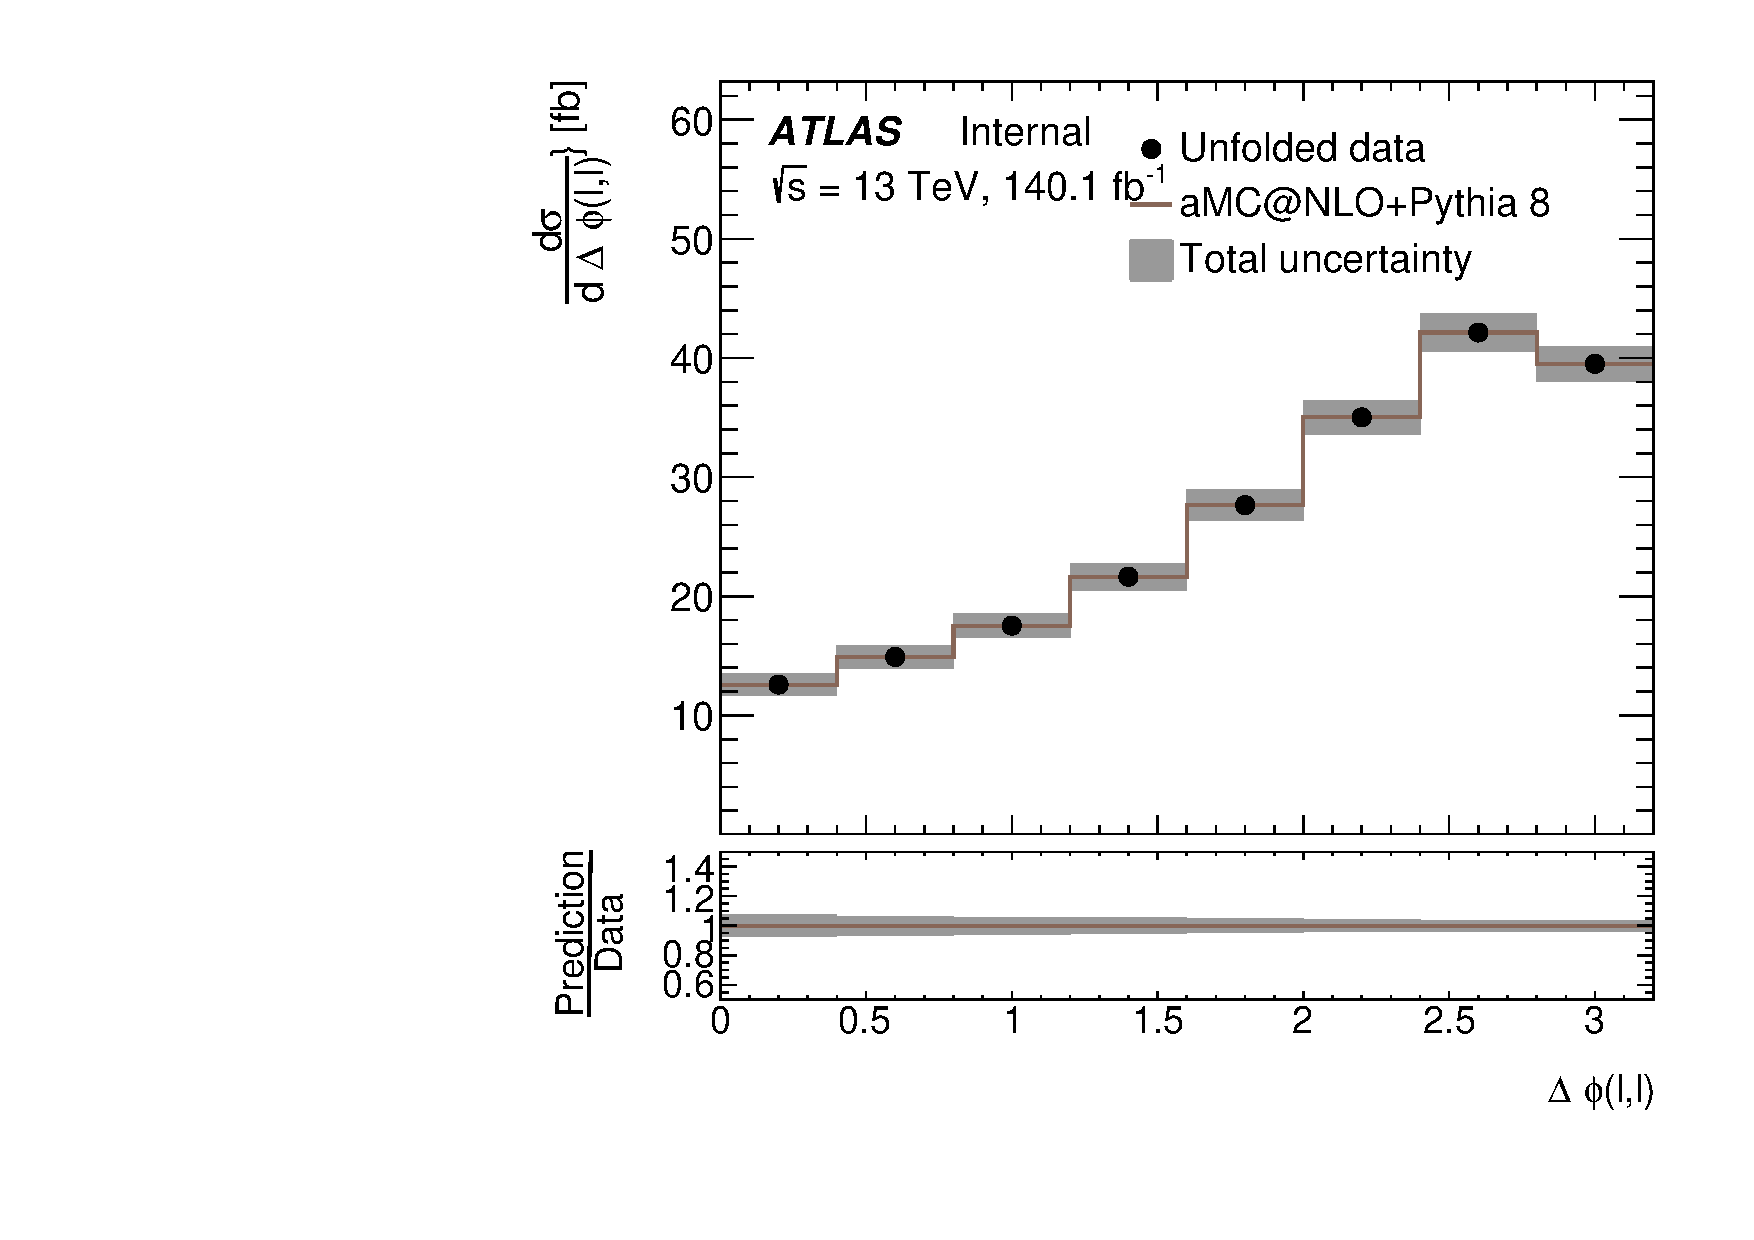
\includegraphics[width=0.23\textwidth]{figures/diff_xsec/binning_optimization/nominal_tty_incl/tty2l_dPhill_all_stat_UnfoldedData.pdf}}
    \hfill
    \subfloat[]{\includegraphics[width=0.23\textwidth]{figures/diff_xsec/binning_optimization/migrations/migration_tty_prod_06/migration_h2_dPhill_reco_part_full_weighted_SR1.pdf}}
    \hfill
    \subfloat[]{\includegraphics[width=0.23\textwidth]{figures/diff_xsec/binning_optimization/migrations/migration_tty_prod_nominal/migration_h2_dPhill_reco_part_full_weighted_SR1.pdf}}
    \hfill
    \subfloat[]{\includegraphics[width=0.23\textwidth]{figures/diff_xsec/binning_optimization/migrations/migration_tty_incl_06/migration_h2_dPhill_reco_part_full_weighted_SR1.pdf}}
    \hfill
    \subfloat[]{\includegraphics[width=0.23\textwidth]{figures/diff_xsec/binning_optimization/migrations/migration_tty_incl_nominal/migration_h2_dPhill_reco_part_full_weighted_SR1.pdf}}
    \hfill

    \caption{(a) Resolution of the photon $|\Delta \phi(l,l)|$ observable is represented by the error bars. The y-axis
    is the mean of (reconstructed photon $|\Delta \phi(l,l)|$ - truth photon $|\Delta \phi(l,l)|$) in GeV and the error bars represent
    one standard deviation around that mean.
    Unfolded results with the tested binning (b) and final
    binning (c) for \tty(prod) measurement and unfolded results with the tested
    (d) and final (e) binning for \tty(total) measurement, The error bar in (b),
    (c), (d), (e) represents statistical uncertainty only.
    The error bar in (b), (c), (d), (e) represents statistical uncertainty only.
    Plots (f)- (i) represents the migration matrix in the SR for above cases.}
\end{figure}
\FloatBarrier

